%%%%%%%%%%%%%%%%%%%%%%%%%%%%%%%%%%%%%%%%%%%%%%%%%%%%%%%%%%%%%%%%%%%%% 
%% This is a (brief) model paper using the achemso class 
%% The document class accepts keyval options, which should include 
%% the target journal and optionally the manuscript type. 
%%%%%%%%%%%%%%%%%%%%%%%%%%%%%%%%%%%%%%%%%%%%%%%%%%%%%%%%%%%%%%%%%%%%% 
\documentclass[journal=jpcbfk,manuscript=article]{achemso} 
 
%%%%%%%%%%%%%%%%%%%%%%%%%%%%%%%%%%%%%%%%%%%%%%%%%%%%%%%%%%%%%%%%%%%%% 
%% Place any additional packages needed here.  Only include packages 
%% which are essential, to avoid problems later. Do NOT use any 
%% packages which require e-TeX (for example etoolbox): the e-TeX 
%% extensions are not currently available on the ACS conversion 
%% servers. 
%%%%%%%%%%%%%%%%%%%%%%%%%%%%%%%%%%%%%%%%%%%%%%%%%%%%%%%%%%%%%%%%%%%%% 

%% Workaround for malfunctioning textsuperscript with pdfx and T1 encoding
\let\tmpa\textsuperscript
\DeclareTextCommandDefault{\textsuperscript}{\tmpa}

\usepackage[x11names]{xcolor}  % typesetting in color
%% Generate PDF/A-2u
%\usepackage[a-2u]{pdfx}
 
\usepackage[super]{natbib}         % citation style AUTHOR (YEAR), or AUTHOR [NUMBER]

\usepackage{achemso}  
\usepackage{rotating}  
%\usepackage{times} 
%\usepackage{lmodern}    %% Prefer Latin Modern fonts
\usepackage{graphicx} 
\usepackage{setspace} 
\usepackage{amsmath} 
\usepackage{epstopdf} 
\usepackage{csquotes} 
\usepackage{mhchem} 
\usepackage{chemfig} 
\usepackage[obeyFinal]{easy-todo}
\usepackage[english]{babel}
\usepackage{xr}
\externaldocument{manuscriptSUPPL}


\usepackage{subfig}
\usepackage{dcolumn}        % improved alignment of table columns
\usepackage{booktabs}       % improved horizontal lines in tables
\usepackage{paralist}       % improved enumerate and itemize

%% Character encoding: usually latin2, cp1250 or utf8:
\usepackage[utf8]{inputenc}
\usepackage[T1]{fontenc}

%\usepackage{markdown}  
 
%% The hyperref package for clickable links in PDF and also for storing
%% metadata to PDF (including the table of contents).
%% Most settings are pre-set by the pdfx package.
%\hypersetup{unicode}
%\hypersetup{breaklinks=true}
%\hypersetup{colorlinks,allcolors=DodgerBlue4}
 
%%%%%%%%%%%%%%%%%%%%%%%%%%%%%%%%%%%%%%%%%%%%%%%%%%%%%%%%%%%%%%%%%%%%% 
%% If issues arise when submitting your manuscript, you may want to 
%% un-comment the next line.  This provides information on the 
%% version of every file you have used. 
%%%%%%%%%%%%%%%%%%%%%%%%%%%%%%%%%%%%%%%%%%%%%%%%%%%%%%%%%%%%%%%%%%%%% 
%%\listfiles 
 
%%%%%%%%%%%%%%%%%%%%%%%%%%%%%%%%%%%%%%%%%%%%%%%%%%%%%%%%%%%%%%%%%%%%% 
%% Place any additional macros here.  Please use \newcommand* where 
%% possible, and avoid layout-changing macros (which are not used 
%% when typesetting). 
%%%%%%%%%%%%%%%%%%%%%%%%%%%%%%%%%%%%%%%%%%%%%%%%%%%%%%%%%%%%%%%%%%%%% 
\newcommand*\mycommand[1]{\texttt{\emph{#1}}} 
%%% Custom variables
% width suitable for fitting into a column in 1-column page layout
\newlength{\figwidth}
\setlength{\figwidth}{9 cm} 
\newlength{\figwidthsmall}
\setlength{\figwidthsmall}{6 cm} 
\newlength{\figwidthfull}
\setlength{\figwidthfull}{14 cm} 
\newlength{\figheightsmall}
\setlength{\figheightsmall}{6 cm} 
\newlength{\figheight}
\setlength{\figheight}{12 cm} 

 
%%%%%%%%%%%%%%%%%%%%%%%%%%%%%%%%%%%%%%%%%%%%%%%%%%%%%%%%%%%%%%%%%%%%% 
%% Meta-data block 
%% --------------- 
%% Each author should be given as a separate \author command. 
%% 
%% Corresponding authors should have an e-mail given after the author 
%% name as an \email command. Phone and fax numbers can be given 
%% using \phone and \fax, respectively; this information is optional. 
%% 
%% The affiliation of authors is given after the authors; each 
%% \affiliation command applies to all preceding authors not already 
%% assigned an affiliation. 
%% 
%% The affiliation takes an option argument for the short name.  This 
%% will typically be something like "University of Somewhere". 
%% 
%% The \altaffiliation macro should be used for new address, etc. 
%% On the other hand, \alsoaffiliation is used on a per author basis 
%% when authors are associated with multiple institutions. 
%%%%%%%%%%%%%%%%%%%%%%%%%%%%%%%%%%%%%%%%%%%%%%%%%%%%%%%%%%%%%%%%%%%%% 
 
\author{Josef Melcr} 
\email{melcr@marge.uochb.cas.cz} 
%%\homepage[]{https://jmelcr.github.io/}
\affiliation{Institute of Organic Chemistry and Biochemistry, 
Academy of Sciences of the Czech Republic,  
Prague 6, Czech Republic} 
\author{Tiago Ferreira}
\affiliation{NMR group - Institut for Physics, Martin-Luther University Halle-Wittenberg} 
\author{Pavel Jungwirth} 
%%\homepage[]{http://jungwirth.uochb.cas.cz/}
\affiliation{Institute of Organic Chemistry and Biochemistry, 
Academy of Sciences of the Czech Republic,  
Prague 6, Czech Republic} 
\alsoaffiliation{Department of Physics, Tampere University of Technology, P.O. Box 692, FI-33101 
Tampere, Finland} 
\author{O. H. Samuli Ollila} 
\email{samuli.ollila@helsinki.fi} 
%%\homepage[]{Your web page} 
\affiliation{Institute of Organic Chemistry and Biochemistry, 
Academy of Sciences of the Czech Republic,  
Prague 6, Czech Republic} 
\alsoaffiliation{Institute of Biotechnology, University of Helsinki} 
 
 
%\author{Andrew N. Other} 
%\altaffiliation{A shared footnote} 
%\author{Fred T. Secondauthor} 
%\altaffiliation{Current address: Some other place, Othert\"own, 
%Germany} 
%\author{I. Ken Groupleader} 
%\altaffiliation{A shared footnote} 
%\email{i.k.groupleader@unknown.uu} 
%\phone{+123 (0)123 4445556} 
%\fax{+123 (0)123 4445557} 
%\affiliation[Unknown University] 
%{Department of Chemistry, Unknown University, Unknown Town} 
%\alsoaffiliation[Second University] 
%{Department of Chemistry, Second University, Nearby Town} 
%\author{Susanne K. Laborator} 
%\email{s.k.laborator@bigpharma.co} 
%\affiliation[BigPharma] 
%{Lead Discovery, BigPharma, Big Town, USA} 
%\author{Kay T. Finally} 
%\affiliation[Unknown University] 
%{Department of Chemistry, Unknown University, Unknown Town} 
%\alsoaffiliation[Second University] 
%{Department of Chemistry, Second University, Nearby Town} 
 
%%%%%%%%%%%%%%%%%%%%%%%%%%%%%%%%%%%%%%%%%%%%%%%%%%%%%%%%%%%%%%%%%%%%% 
%% The document title should be given as usual. Some journals require 
%% a running title from the author: this should be supplied as an 
%% optional argument to \title. 
%%%%%%%%%%%%%%%%%%%%%%%%%%%%%%%%%%%%%%%%%%%%%%%%%%%%%%%%%%%%%%%%%%%%% 
%\title[] 
%  {Accurate interactions of cations with 
%   neutral and negatively charged membranes 
%   via combination of experiments and molecular simulation}

\title[] 
{Improved Cation Binding to Lipid Bilayer with Negatively Charged POPS by Effective Inclusion of Electronic Polarization}
  %Detailed structure of negatively charged membranes 
  %  of phosphatidylserine and phosphatidylcholine 
  %  at concentrations of calcium, sodium and potassium salts
  %  from molecular dynamics simulations with electronic polarization }
  % JOSEF: I feel that the above title is a bit better, because it focuses on PS,
  %        but the following one is an alternative, which focuses more on the cations as in roux90
  %{ Detailed structure of calcium, sodium and potassium cations
  %  at negatively charged membranes of phosphatidylserine and phosphatidylcholine 
  %  from molecular dynamics simulations with electronic polarization }

%%%%%%%%%%%%%%%%%%%%%%%%%%%%%%%%%%%%%%%%%%%%%%%%%%%%%%%%%%%%%%%%%%%%% 
%% Some journals require a list of abbreviations or keywords to be 
%% supplied. These should be set up here, and will be printed after 
%% the title and author information, if needed. 
%%%%%%%%%%%%%%%%%%%%%%%%%%%%%%%%%%%%%%%%%%%%%%%%%%%%%%%%%%%%%%%%%%%%% 
\abbreviations{IR,NMR,UV,MD,ECC,PC,PS,POPS,POPS} 
\keywords{MD simulation, molecular modeling, 
          polarizability, polarization,
          phospholipids, phosphatidylserine} 

%%%%%%%%%%%%%%%%%%%%%%%%%%%%%%%%%%%%%%%%%%%%%%%%%%%%%%%%%%%%%%%%%%%%% 
%% The manuscript does not need to include \maketitle, which is 
%% executed automatically. 
%%%%%%%%%%%%%%%%%%%%%%%%%%%%%%%%%%%%%%%%%%%%%%%%%%%%%%%%%%%%%%%%%%%%% 
\begin{document} 
 
%%%%%%%%%%%%%%%%%%%%%%%%%%%%%%%%%%%%%%%%%%%%%%%%%%%%%%%%%%%%%%%%%%%%% 
%% The "tocentry" environment can be used to create an entry for the 
%% graphical table of contents. It is given here as some journals 
%% require that it is printed as part of the abstract page. It will 
%% be automatically moved as appropriate. 
%%%%%%%%%%%%%%%%%%%%%%%%%%%%%%%%%%%%%%%%%%%%%%%%%%%%%%%%%%%%%%%%%%%%% 
\begin{tocentry} 
 
Some journals require a graphical entry for the Table of Contents. 
This should be laid out ``print ready'' so that the sizing of the 
text is correct. 
 
Inside the \texttt{tocentry} environment, the font used is Helvetica 
8\,pt, as required by \emph{Journal of the American Chemical 
Society}. 
 
The surrounding frame is 9\,cm by 3.5\,cm, which is the maximum 
permitted for  \emph{Journal of the American Chemical Society} 
graphical table of content entries. The box will not resize if the 
content is too big: instead it will overflow the edge of the box. 
 
This box and the associated title will always be printed on a 
separate page at the end of the document. 
 
\end{tocentry} 
 
%%%%%%%%%%%%%%%%%%%%%%%%%%%%%%%%%%%%%%%%%%%%%%%%%%%%%%%%%%%%%%%%%%%%% 
%% The abstract environment will automatically gobble the contents 
%% if an abstract is not used by the target journal. 
%%%%%%%%%%%%%%%%%%%%%%%%%%%%%%%%%%%%%%%%%%%%%%%%%%%%%%%%%%%%%%%%%%%%% 
 
 
 
\begin{abstract} 
  Phosphatidylserine (PS) lipids are important signaling molecules and the most common negatively charged lipids in eukaryotic membranes.
  The signaling can be often regulated with calcium, but its interactions with PS headgroups are not fully understood.
  Classical molecular dynamics (MD) simulations can potentially give detailed description of lipid-ion interactions,
  but the results strongly depend on the used force field.
  Here, we apply the electronic continuum correction (ECC) to the Amber Lipid17 parameters of POPS lipid to improve its
  interactions with Na$^+$ and Ca$^{2+}$ ions.
  The partial charges of headgroup, glycerol backbone and carbonyls of POPS, bearing a unit negative charge, were scaled with a
  factor of 0.75, derived for monovalent ions and the Lennard-Jones $\sigma$ parameters of the same segments were scaled with a factor of 0.89.
  The resulting ECC-POPS models, gives more realistic interactions with Na$^+$ and Ca$^{2+}$ cations than the original Amber Lipid17 parameters,
  when validated using the headgroup order parameters and ''electrometer concept''.
  In ECC-lipids simulations, the Ca$^{2+}$ cations do not simultaneously interact with more than two PS lipids, and interactions 
  carboxylate groups is twice more likely than with phosphate group, while interaction with carbonyls is almost negligible.
  Our results pave the way for more realistic MD simulations of anionic biological membranes and demonstrate the ECC
  approach is useful also for charged lipids.
\end{abstract} 
 
 
%\begin{abstract} 
%  This is an example document for the \textsf{achemso} document 
%  class, intended for submissions to the American Chemical Society 
%  for publication. The class is based on the standard \LaTeXe\ 
%  \textsf{report} file, and does not seek to reproduce the appearance 
%  of a published paper. 
 
%  This is an abstract for the \textsf{achemso} document class 
%  demonstration document.  An abstract is only allowed for certain 
%  manuscript types.  The selection of \texttt{journal} and 
%  \texttt{manuscript} will determine if an abstract is valid.  If 
%  not, the class will issue an appropriate error. 
%\end{abstract} 
 
%%%%%%%%%%%%%%%%%%%%%%%%%%%%%%%%%%%%%%%%%%%%%%%%%%%%%%%%%%%%%%%%%%%%% 
%% Start the main part of the manuscript here. 
%%%%%%%%%%%%%%%%%%%%%%%%%%%%%%%%%%%%%%%%%%%%%%%%%%%%%%%%%%%%%%%%%%%%% 
 
 
 
\section{Introduction} 

Phosphatidylserine (PS) lipids are the most common negatively charged lipids in eukaryotic membranes
and important signaling molecules \cite{lemmon08,leventis10,li14}.
They interact with signaling proteins \cite{leventis10},
regulate surface charge and protein localization \cite{yeung08}, 
induce protein aggregation \cite{zhao04,gorbenko06} and membrane fusion \cite{??}.
Because these functions are also often regulated by biological cations \cite{leventis10},
the detailed interactions between PS lipids and biological cations, like calcium, are under great interest.
\todo{Pavel can probably improve and complement this}

%Various interaction schemes have been proposed for the negatively charged
%lipids with ions and other lipids. 
Spectroscopic experiments give detailed information about the
interactions between ions and PS lipids, but the data is often indirect and difficult to
interpret \cite{hauser77,kurland79,eisenberg79,hauser83,dluhy83,hauser85,feigenson86,mattai89,roux90,roux91}.
Some studies suggest that the
binding constant of ions to negatively charged lipids is similar to that of zwitterionic lipids,
and the binding affinity is increased only due to the increased cation
concentration in the vicinity of the membrane \cite{seelig90,sinn06}.
On the other hand, calcium forms dehydrated complexes with PS headgroups
which cause phase separation \cite{hauser77,kurland79,hauser85,feigenson86,mattai89,roux90,roux91,boettcher11}.
Theories about the interaction between calcium and PS 
are difficult to evaluate experimentally,
especially at physiological ion concentrations,
which are typically too low to yield measurable effects.

More recently, classical molecular dynamics (MD) simulations
have been used to support the interpretation of spectroscopic experiments,
but the results strongly depend on the force field parameters \cite{boettcher11,kucerka14,melcrova16,hallock18,valentine18}.
% smoother connection between previous and following statements
For instance, the moieties of PS lipids that interact with calcium cations vary greatly.
In simulations with the CHARMM36 force field \cite{klauda10,venable13} using the NBfix parameters for calcium \cite{kim16}, 
calcium ions interact only with the carboxylate group of PS lipids \cite{valentine18}.
However, the same force field without the NBfix parameters, gives a significant binding affinity also to the phosphate region \cite{hallock18}.
On the other hand, simulations with the Berger force field \cite{berger97,mukhopadhyay04}
suggest a significant calcium binding also to the carbonyls in the acyl chains \cite{melcrova16}.

The NMRlipids project \url{nmrlipids.blogspot.fi} has recently demonstrated
that such controversies can be resolved by using the headgroup order parameters
of phosphatidylcholine (PC) lipids \cite{catte16, NMRlipidsIV}, which can
be related to cation binding affinity to lipid bilayers using the electrometer
concept \cite{akutsu81,altenbach84,seelig87}. The main advantage of the approach
is the direct comparison between experimental and calculated order parameters,
which reduced the ambiguity arising from the interpretation of the data.
Unfortunately, none of the readily available force fields was sufficiently accurate to correctly reproduce the
cation binding affinity to zwitterionic PC bilayers \cite{catte16} or to the
mixtures with negatively charged PS lipids \cite{NMRlipidsIV}.
In our recent work~\cite{melcr18}, we were able to improve the cation binding affinity
to zwitterionic 1-palmitoyl-2-oleoyl-sn-glycero-3-phosphocholine (POPC) lipid bilayer
by implicitly including electronic polarizability using the electronic continuum
correction (ECC) \cite{leontyev09}. The good agreement between the resulting ECC-POPC
model and experiments enable detailed interpretation of calcium binding details to POPC lipid bilayer.

%There are force field parameters for neutral lipids PC and PE 
%with explicit polarizability using the Classical Durde model. \cite{chowdhary13, chowdhary17}
%While such a model shows a potential improvement over non-polarizable force fields from many perspectives -- 
%for example accounting for polarizability has a significant impact on the dipole potential of a membrane \cite{harder2009} -- 
%the non-polarizable version of the same force field 
%performes comparably well at a fraction of the computational cost 
%of the models with explicit polarization. \citep{lucas12,chowdhary13} 

Here, we extend the ECC approach also to the negatively charged 1-palmitoyl-2-oleoyl-sn-glycero-3-phospho-L-serine (POPS) lipid.
We also complement the available experimental data for the force field quality
evaluation by measuring the acyl chain C--H bond order parameters of POPS in bilayer using natural abundance $^{13}$C NMR.
In addition to the acyl chain order parameters measured here, the quality of the newly developed ECC-POPS force field parameters is
evaluated using previously published C--H bond order parameters of glycerol backbone and headgroup in various ionic
conditions and lipid molar fractions \cite{roux90,NMRlipidsIV}, as well as X-ray scattering form factors\cite{kucerka14}.
The overall improvement of the force field accuracy upon applying ECC
%not only describes the interactions of PS with ions more accurately, 
%but also improves the structure of the PS head group 
%and its interactions with PC in mixed lipid bilayers. 
%The results
paves the way to more realistic MD simulations 
of both neutral and negatively charged lipid bilayers 
for a wide range of applications.

%Here, we demonstrate that the same approach 
%significantly improves the description of calcium binding 
%also to the negatively charged PC:PS (5:1) bilayers. 
%In correspondence with the Ref.~\citenum{NMRlipidsIV},
%we also use the changes of the head group order parameters $S^\alpha$ and $S^\beta$ 
%in PC and PS lipids 
%to quantify the binding affinity of the calcium cations
%and the induced structural changes
%(Fig.~\ref{fig:delta_ordPar_CaCl_PCPS}). 
%To directly connect to the previous works \citep{catte16, NMRlipidsIV}
%and to mark the improvement after treating electronic polarizability, 
%we show simulation results from the newly developed ECC-lipids and also from Lipid17 \citep{lipid17-future}. 

%An empirical scaling factor, which reduces electrostatic forces between molecules, 
%is a well known concept in molecular modelling;
%such an approach was adopted in the early simulations of lipid bilayers \cite{egberts94, berendsen1996},
%in force fields employing explicit polarization \cite{lemkul2016empirical},
%or in the simulations of ionic liquids \cite{Bhargava2007}. 
%%An improvement of permeability of charged solutes in the gramicidin A channel 
%%is observed with a force field using charge equilibration to model polarizability. \cite{lucas2012} 
%At the same time, 
%the implicit inclusion of electronic polarizability to lipid models
%via charge re-scaling using electronic continuum correction (ECC) 
%substantially improved the interactions between cations and zwitterionic lipids \cite{melcr18}. 





 
\section{Methods} 
 
\subsection{Electronic continuum correction for PS lipids}\label{section:ecc} 

Electronic continuum correction (ECC) is an implicit mean-field representation of 
the electronic polarization in classical MD simulations. 
For simple ions in water, the electronic polarizability
can be taken into account by scaling the charge with a constant factor 
%\begin{equation}
 \mbox{$ f_q = \frac{1}{\sqrt{\epsilon_{el}}} \approx 0.75$,}
%\end{equation}
where  $\epsilon_{el} = 1.78$ is the high-frequency dielectric constant of electrons in water \cite{leontyev09}.
The scaling of charges with this factor has been recently applied to improve classical models for ions and
other biomolecules \cite{Pluharova2014, martinek17, duboue2018insulin, Mason2019, Duboue2018MgZn} \todo{Pavel can probably update this (insulin?)}.
In addition to the charge, the Lennard-Jones~$\sigma$ was scaled with a factor $f_\sigma \leq 1$
to improve the hydration properties of ions with respect to scattering data in these studies
\todo{Pavel can probably deliver the state of the art information about these parameters and sharpen the discussion}.

Derivation of the correct scaling factor for lipids is more complicated, because
the partial charges depend on the methods used to derive the respective force fields.
For example, the partial charges may already include the effects of electronic polarizability to some extent,
and hence, the scaling factor can be larger than the theoretically derived value for ions in water, $f_q \approx 0.75$.
Before the ECC theory was rigorously derived, similar idea was already employed in early classical 
MD simulations of lipids and surfactants using the scaling factor of 0.5 for atomic charges  \cite{jonsson86,egberts94, berendsen1996}. 
In our recent work, we applied the ECC to the Amber based lipid14 force field of zwitterionic POPC lipid \cite{dickson14}
by scaling the partial charges and Lennard-Jones~$\sigma$ parameters of headgroup, glycerol backbone,
and carbonyl regions \cite{melcr18}. The scaling factors were optimized to reproduce 
the calcium binding affinity to POPC lipid bilayers, evaluated using the headgroup order parameters
and the electrometer concept \cite{akutsu81,altenbach84,seelig87,catte16}, and the X-ray scattering form factor
without additional ions \cite{kucerka11}, which resulted to the scaling factor values of $f_q = 0.8$ and $f_\sigma = 0.89$  \cite{melcr18}.

Here, we apply the ECC to the Amber-based lipid17 parameters \cite{lipid17-future} of POPS lipid with a monovalent negative charge.
Because POPS carries a physical total charge as aqueous ions, we apply the theoretically derived scaling factor for
ions $f_q = 0.75$ \cite{leontyev09} to the partial charges of POPS. 
The lipids with a total charge of -0.75 are also neutralized
by the counterion charges of +0.75 in simulations with ECC-ions \cite{Pluharova2014, kohagen16, martinek17}.
Following our previous work for POPC, we use the scaling factor of $f_\sigma = 0.89$ for the Lennard-Jones~$\sigma$ parameters and
use it to scale the parameters of atoms only in the headgroup, glycerol backbone, and carbonyl regions \cite{melcr18}.
Further optimization of parameters was not done in this work. 
The generated ECC-POPS parameters are available from Ref.~\citenum{??}
\todo{We need here a permanent citation with DOI.
  Easiest would be to add the parameters into a one of the existing Zenodo repositories containing other simulation parameters.
  We could also put a release of Git into Zenodo, cite that and specify the exact directory where parameters are found,
  but this is more complicated for users to find.
}


\subsection{Measurements of acyl chain order parameters}
A R-type Proton Detected Local Field (R-PDLF) experiment was performed to determine C--H bond order
parameters
\begin{equation}\label{OPequation}
  S_{\rm{CH}}=\frac{1}{2}\langle3\cos^2\theta-1\rangle,
\end{equation}
  where $\theta$ denotes the angle of the C--H bond
with the bilayer normal and the angular brackets define a time average on a time scale of approximately 1 microsecond.
The experiment was done using a Bruker Avance III 400 spectrometer operating at a 1H Larmor frequency of 400.03 MHz
equipped with a standard 4~mm CP-MAS HXY probe. The set up of the R-PDLF experiment was the following
(using the notation from figures 1c and 2c in the original publication describing the R-PDLF experiment \cite{dvinskikh04}).
The magic angle spinning (MAS) frequency used was 5.15 kHz. The recoupling pulses in the R18 blocks had
therefore a length of $10.79 \, \mu \mathrm{s}$, which correspond to a nutation frequency of 46.35~kHz. Increments of $18 \times 2$ recoupling
pulses where used giving a spectral width of 2.6~kHz in the indirect dimension and a total number of 32 points in
the indirect dimension were recorded. These settings enable to record dipolar slices with a C--H bond order parameter
resolution of $\pm$0.01. The C--H bond order parameter determined from a given dipolar
splitting, $\Delta\nu$ (see e.g. Fig. \ref{R-PDLFslices} in \todo{Is this the correct figure?}) is equal to $\Delta\nu/(0.315\times21.5 kHz)$, where 0.315 is
the scaling factor of the R18 recoupling sequence and 21.5 kHz is the maximum $^1$H-$^{13}$C dipolar coupling for a C--H bond.
The refocused-INEPT transfer \cite{morris79,burum80} %[G. Morris and R. Freeman, J. Am. Chem. Soc. 101, 760 (1979);
was used for transferring the polarization from $^1$H nuclei to the covalently bond $^{13}$C nuclei with the delays $\tau_1 = 1.94$~ms and $\tau_2 = 0.97$~ms
(set as multiples of the MAS rotation period). The pulses for the refocused-INEPT sequence had a nutation frequency equal to 63.45~kHz.
For acquiring the spectra, a total number of 1024 transients were recorded for each point in the indirect dimension, using an acquisition
time of 0.1~s under SPINAL64 $^1$H decoupling \cite{fung00} with a nutation frequency of 50~kHz, and with dwell time giving a spectral
width of 200 ppm for the $^{13}$C chemical shift dimension. The set of free induction decays recorded were then processed as
described e.g. in Ref.~\citenum{ferreira08}. The dipolar splittings in the crowded spectral region
between 29 and 30 ppm were assigned based on the previous assignments for POPC \cite{ferreira13} 
and the POPS order parameters calculated from simulations in this work.
 
\subsection{Simulation details} 


\begin{table*}[tbp]
\centering
\caption{  List of MD simulations reporting their respective
           lipid composition,
           used counterions,
           added buffer concentrations,
           amounts of individual molecules,
           and the deployed models.
           The fatty acid chains for all lipids are palmitoyl (sn-1) and oleoyl (sn-2).
         }\label{tbl:sim-list}
\begin{tabular}{r  l | r r r r | r r | c c }
   \multicolumn{1}{r}{PC:PS} & \multicolumn{1}{l}{ }  &  \multicolumn{4}{c}{added buffer conc. / mM}    & \multicolumn{2}{c}{no. molecules} &  \multicolumn{2}{c}{simulated with}  \\
   ratio & counterion &  \ce{K^+}  &  \ce{Na^+} & \ce{Ca^{2+}} & \ce{Cl^-}      & \ce{H2O} &  PC:PS                 &  ECC-lipids  &  Lipid17    \\
  \hline
only PS & \ce{K^+}   &      0  &      0  &      0  &      0  &  3600  &  0:72  &  \textbullet &  \textbullet \\ 
only PS & \ce{Na^+}  &      0  &      0  &      0  &      0  &  3600  &  0:72  &  \textbullet &  \textbullet \\ 
  \hline
1:1 & \ce{K^+}   &      0  &      0  &      0  &      0  &  5253  &  64:64  &  \textbullet &  \textbullet \\ 
1:1 & \ce{Na^+}  &      0  &      0  &      0  &      0  &  5253  &  64:64  &  \textbullet &  \textbullet \\ 
  \hline
4:1 & \ce{K^+}   &      0  &      0  &      0  &      0  &  3600  &  48:12  &  \textbullet &  -  \\ 
4:1 & \ce{Na^+}  &      0  &      0  &      0  &      0  &  3600  &  48:12  &  \textbullet &  -  \\ 
  \hline
5:1 & \ce{K^+}   &      0  &      0  &      0  &      0  &  3600  &  60:12  &  \textbullet &  \textbullet \\ 
5:1 & \ce{Na^+}  &      0  &      0  &      0  &      0  &  3600  &  60:12  &  \textbullet &  \textbullet \\ 
5:1 & \ce{Na^+}  &      0  &      0  &     78  &     78  &  3561  &  60:12  &  \textbullet &  \textbullet \\ 
5:1 & \ce{Na^+}  &      0  &      0  &    125  &    125  &  3561  &  60:12  &  \textbullet &  \textbullet \\ 
5:1 & \ce{Na^+}  &      0  &      0  &    202  &    202  &  3561  &  60:12  &  \textbullet &  \textbullet \\ 
5:1 & \ce{Na^+}  &      0  &      0  &    409  &    409  &  3522  &  60:12  &  \textbullet &  \textbullet \\ 
5:1 & \ce{Na^+}  &      0  &      0  &    621  &    621  &  3483  &  60:12  &  \textbullet &  \textbullet \\ 
5:1 & \ce{Na^+}  &      0  &    621  &      0  &    621  &  3483  &  60:12  &  \textbullet &  \textbullet \\ 
5:1 & \ce{Na^+}  &      0  &   1510  &      0  &   1510  &  3377  &  60:12  &  \textbullet &  \textbullet \\ 
5:1 & \ce{Na^+}  &      0  &   3002  &      0  &   3002  &  3213  &  60:12  &  \textbullet &  \textbullet \\ 
5:1 & \ce{Na^+}  &    621  &      0  &      0  &    621  &  3483  &  60:12  &  \textbullet &  \textbullet \\ 
5:1 & \ce{Na^+}  &   1510  &      0  &      0  &   1510  &  3377  &  60:12  &  \textbullet &  \textbullet \\ 
5:1 & \ce{Na^+}  &   3002  &      0  &      0  &   3002  &  3213  &  60:12  &  \textbullet &  \textbullet \\ 
  \hline
10:1 & \ce{K^+}  &      0  &      0  &      0  &      0  &  3600  &  60:6  &  \textbullet &  -  \\ 
10:1 & \ce{Na^+} &      0  &      0  &      0  &      0  &  3600  &  60:6  &  \textbullet &  -  \\ 
\end{tabular}
\end{table*}


MD simulations of POPC:POPS lipid bilayers with different molar ratios 
and ion concentrations (\ce{K^+}, \ce{Na^+}, \ce{Ca^{2+}} and \ce{Cl^{-}})
were performed in an orthorhombic simulation box with periodic boundary conditions
using the GROMACS 2018 \cite{Abraham15} simulation package. 
The simulated systems are listed in Table~\ref{tbl:sim-list}
and the used simulation parameters in Table~\ref{tbl:mdpar}. 
All simulations were ran for a minimum of $1 \, \mu$s,
and the first  $50 \,$ns were omitted as an equilibration period. 
For deposited trajectories and parameter files see 
Refs.~\citenum{ecclipids_pcps_nacl_kcl_series, ecclipids_pcps_cacl2_series, ecclipids_pcps_mixtures_counterions, 
               lipid17_nacl_kcl_series, lipid17_ff99_ions, lipid17_cacl_series}

In the reference simulations with the standard Amber force field,
the Lipid14 parameters~\cite{dickson14} for POPC, the Lipid17 parameters for POPS \cite{lipid17-future},
the TIP3P water model~\cite{jorgensen83}, and ion models by Dang and coworkers~\cite{smith94,chang1999,dang2006} were used.
The previously generated \cite{botan15} Lipid14 parameters for POPC in Gromacs format were downloaded from Ref.~\citenum{lipid14files}. 
The Lipid17 parameters for POPS were obtained from AmberTools18 \cite{amber18} 
and converted to Gromacs format using acpype \cite{acpype}.  
The ion model by Dang and coworkers~\cite{smith94,chang1999,dang2006} was used with Amber lipids because
the default Amber ion parameters \cite{aqvist90} led to the artificial clustering of ions in solution \cite{NMRlipidsIV}.
In the ECC-lipids simulations,
the ECC-POPC parameters~\cite{melcr18} (available from Ref. \citenum{ECC-POPC_nacl_cacl2_files}), 
the ECC-POPS parameteres derived in this work (see above), 
the SPC/E~\cite{Berendsen1987} water model, and ECC-ions \cite{martinek17, kohagen16, Pluharova2014} were used.
The SPC/E water model was selected because its lower dielectric constant is consistent with the
ECC concept \cite{leontyev11,leontyev14}.
\begin{table}[tbp]
  \caption{Simulation parameters}
  \label{tbl:mdpar}
  \begin{tabular}{ll}
    simulation property & parameter   \\
    \hline
    time-step           & 2~fs         \\
    equilibration time  & 50~ns  \\
    total simulation time     & $\geq 1 \mu$s  \\
    temperature         & 298~K       \\
    thermostat          & v-rescale  \cite{bussi07}   \\
    barostat            & Parrinello-Rahman, semi-isotropic \cite{parrinello81} \\
    long-range electrostatics & PME  \cite{darden93}  \\
    cut-off scheme      & Verlet \cite{Pall13}      \\
    Coulomb and VdW cut-off & 1.0~nm \\
    constraints         & LINCS, only hydrogen atoms \cite{hess97} \\
    constraints for water & SETTLE  \cite{miyamoto92} \\
    \hline
  \end{tabular}
\end{table}
 
The C--H bond order parameters were calculated directly from Eq.~\ref{OPequation}.
The time average was first calculated for each lipid, and
the standard error of the mean from these individual values was then used as the
error estimate \cite{botan15,ollila16,NMRlipidsIV}.
Python program that uses the
MDAnalysis library \cite{agrawal11,gowers16} is available in Ref.~\citenum{MATCHgit} ({\tt scripts/calcOrderParameters.py}). 
The ion number density profiles were calculated using the {\tt gmx density} tool
of the Gromacs sofware package \cite{gromacsMANUAL}.
The salt concentrations in buffer before solvating the lipids, reported in the used experimental data set \cite{roux90},
were calculated as $[{\rm salt}]=N_{\rm c} \times[{\rm water}]\,/\,N_{\rm w}$,
where $N_{\rm c}$ is the number of cations in simulation, $[{\rm water}]$\,=\,55.5~M and $N_{\rm w}$
is the number of water molecules in the simulation.
As discussed in our previous work \cite{NMRlipidsIV}, the hydration levels of
multilamellae are expected to be sufficiently similar in the used simulations and reference experiments \cite{roux90}.









% ++++++++++++++++++++++++++++++++++++++++++++++++++++++++++++++++++++++++++++++++++++
% ++++++++  RESULTS AND DISCUSSION section +++++++++++++++++++++++++++++++++++++++++++
% ++++++++++++++++++++++++++++++++++++++++++++++++++++++++++++++++++++++++++++++++++++

\section{Results and Discussion} 
 
\subsection{ECC-POPS improves agreement in experimental structural parameters of a pure POPS bilayer } 
 
The X-ray scattering form factors and C-H bond order parameters from NMR experiments are good measures to validate
the lipid bilayer structure in MD simulations against experiments because they
are related to the bilayer dimensions (area per molecule and thickness) and
conformational fluctuations of individual lipids, respectively, and 
can be directly calculated from MD simulations~\cite{ollila16}.
The X-ray scattering form factors and C-H bond order parameters in
the headgroup and glycerol backbone region of a POPS lipid bilayer are already available in the literature \cite{kucerka14,NMRlipidsIV}.
Here, we measure also the C--H bond order parameters of the acyl chain region using natural abundance $^{13}$C NMR.
We first determined the order parameters of each peak corresponding to different C--H bonds detected
in the first dimension (Fig.~\ref{R-PDLF}) from the dipolar slices in the indirect dimension (Fig.~\ref{R-PDLFslices}).
Because the exact assignment of these peaks was not possible, we assigned the
acyl chain order parameters to mimic the profile predicted by the MD simulations (Fig.~\ref{simVSexpNOions_POPS}).
\todo{Tiago should check and update this and figures in SI.}


\begin{figure}[tb!] 
  \centering 
  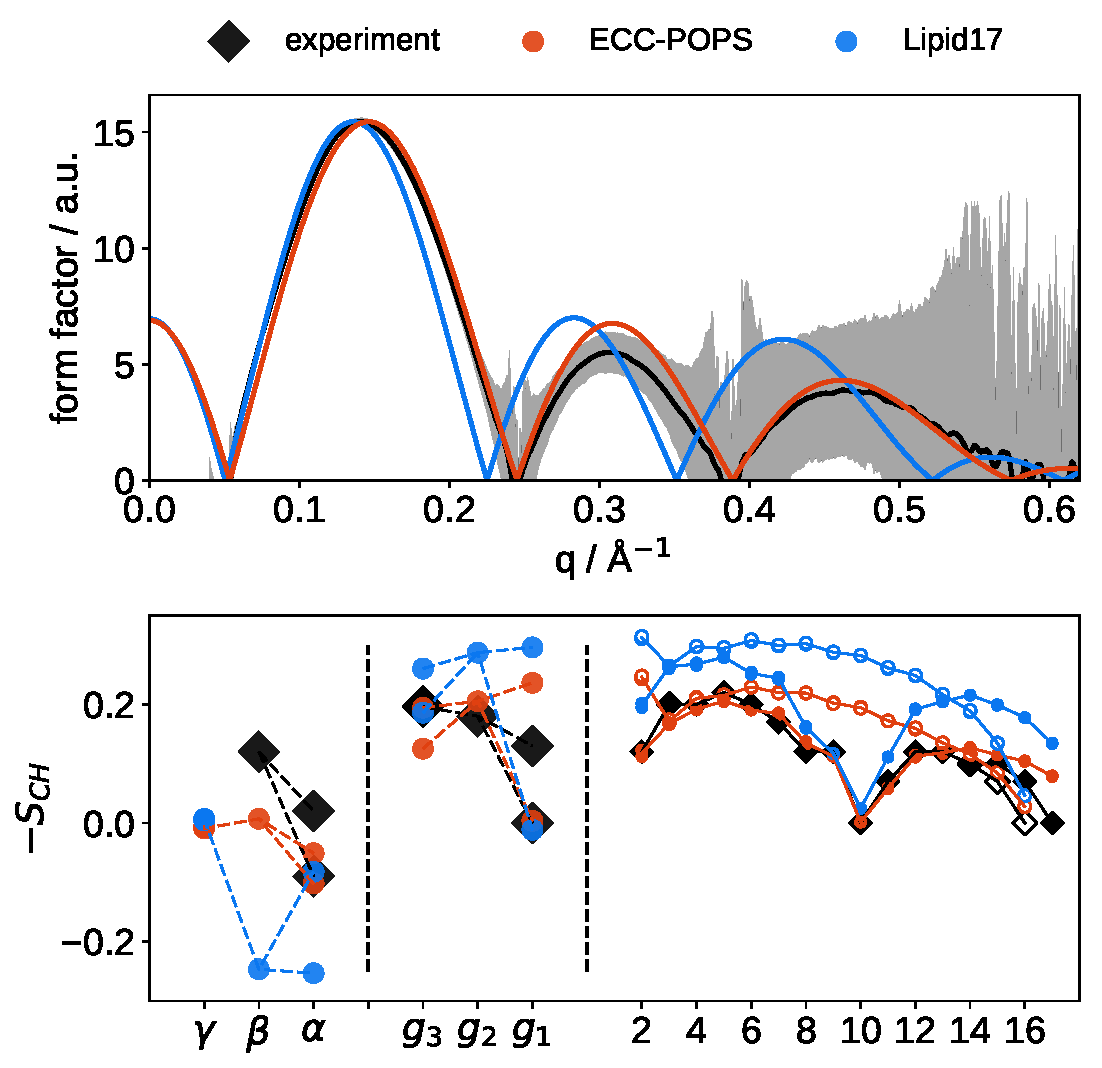
\includegraphics[width=\figwidth]{../img/ecc_pops/Order-parameters_form-factors_exp-L17-ECC-lipids.pdf}
  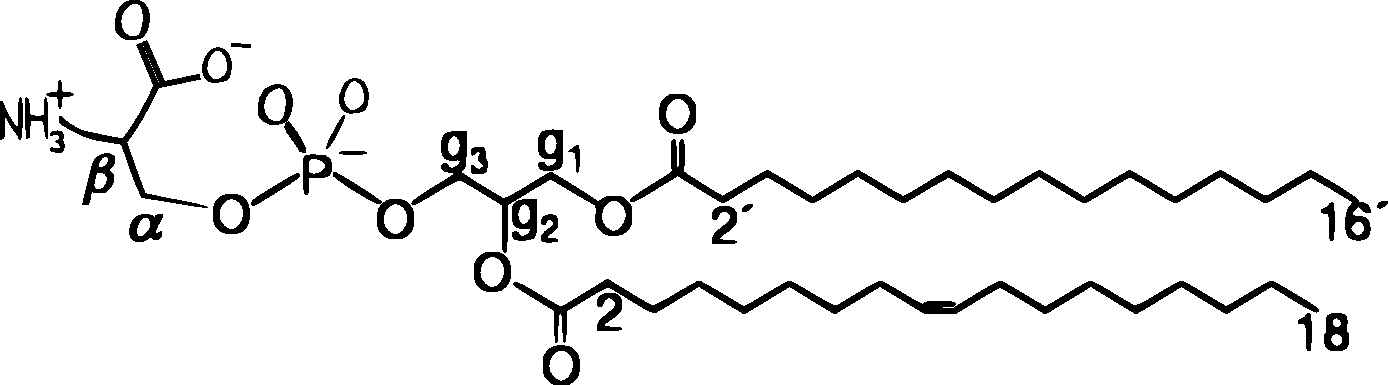
\includegraphics[width=\figwidth]{../img/POPSstructure.pdf} 
\hfill
  \caption{\label{simVSexpNOions_POPS} 
    \textbf{Top:} X-ray scattering form factors from simulations with Lipid17/Dang \citep{lipid17-future, dang2006} and 
    ECC-POPS/ECC-ions \cite{martinek17, Pluhackova2016} compared with experiments~\citep{kucerka14} at 298~K. 
    \textbf{Middle:} Order parameters of POPS head group, glycerol backbone and acyl chains  
    from the same simulations 
    compared with experiments at 298~K. \citep{NMRlipidsIV}
    Open/closed symbols are used for palmitoyl/oleoyl chains of POPS. 
    \textbf{Bottom:} The chemical structure of POPS and the labeling of the carbon segments. 
  }  
\end{figure} 


The Lipid17/Dang simulation gives 
discrepancies with the experimental X-ray form factor,
larger acyl chain order parameters,
and smaller area per molecule than the experimental values (Fig.~\ref{simVSexpNOions_POPS} and table~\ref{tab:apls}),
indicating that this simulation predicts a too compact POPS lipid bilayer. 
The ECC-POPS simulation gives better agreement with experiments for the X-ray scattering form factors and 
acyl chain order parameters (Fig.~\ref{simVSexpNOions_POPS}),
indicating that the bilayer dimensions and acyl chain
conformations are well described by the force field. The area per lipid from ECC-POPS simulation is slightly
smaller than the value reported from SDP model \cite{kucerka14} (table~\ref{tab:apls}), but the values
agree within their error estimates. The larger area in ECC-POPS simulation can be
explained by increased headgroup repulsion due to lower counterion binding affinity (Fig. \ref{fig:POPS-counterions-dens}).
This explains also the larger area per molecule (57~\AA$^2$) reported for Lipid17 POPS simulations
%being closer to the experimental value, 
%In previous study \cite{NMRlipidsIV}, the Lipid17 force field
with {\AA}qvist ions~\cite{NMRlipidsIV}.
%gave a 
%which is probably due to the weaker counterion binding affinity of {\AA}qvist ions to phospholipids. \cite{catte16, NMRlipidsIV}
However, the Dang ions %with more realisitic bulk properties
are used here to analyze the effect of ECC to the properties of a POPS lipid bilayer because
{\AA}qvist ions produce known artifacts, like artificial aggregation of ions at larger salt concentrations \cite{kohagen16, chen07, NMRlipidsIV}.

%SAMULI: I have moved this figure back to the main text
\begin{figure}[hbp!] 
  \centering 
  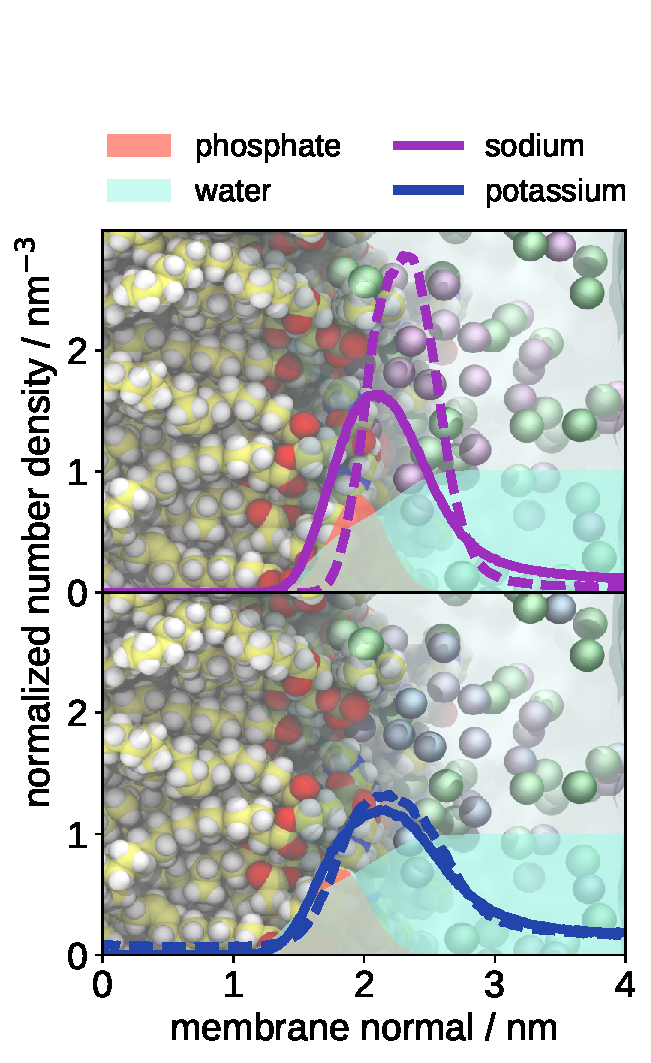
\includegraphics[width=8cm]{../img/ecc_pops/density_profiles_na-k-counterions_wat_phos_compar_purePOPS_ecclipids-lipid17.pdf}
  \caption{\label{fig:POPS-counterions-dens}
    Number density profiles of \ce{K^{+}} and \ce{Na^{+}} counterions along the membrane normal axis
    in ECC-lipids (solid lines) and Lipid17/Dang (dashed lines) simulations of pure POPS bilayers.  
    The density profiles of phosphate groups and water are divided by 4 and 100, respectively.  
  }
  \todo{This figure might be more clear without the lipids in background.}
\end{figure}



\begin{table}[tb!] 
\centering
  \caption{Area per lipid of POPS bilayers, $A_L$, from simulations with different force fields at 298~K with \ce{Na^+} counterions. \label{tab:apls} } 
  \begin{tabular}{l|c } 
    \multicolumn{2}{c}{POPS} \\
    model          & $A_L$ / Å$^2$    \\ 
    \hline 
    Lipid17/Dang              & 53.5$\pm$ 1.7   \\ 
%    Lipid17/ff99              & 57.9$\pm$ 1.7   \\ 
%    \hline 
    ECC-POPS/ECC-ions         & 59.8$\pm$ 1.8   \\ 
%    \hline 
    experiment (SDP model) \citep{kucerka14} & 62.7$\pm$ 1.3  \\ 
%    \hline 
  \end{tabular} \\
\todo{J: This table will become a small inset plot in the top of Fig.~\ref{simVSexpNOions_POPS} }
\end{table} 

Despite the success in simulating bilayer dimensions and acyl chain conformations,
lipid force fields have typically problems in capturing the correct glycerol backbone and
headgroup order parameters and conformations \cite{botan15,ollila16,NMRlipidsIV}.
This is the case also for Lipid17 POPS simulations, where the headgroup and glycerol backbone
order parameters are quite far from experimental values with Dang (Fig.~\ref{simVSexpNOions_POPS}),
{\AA}qvist and Joung-Cheatham ions~\cite{NMRlipidsIV}. The values from ECC-POPS simulation are closer,
but not in full agreement with experiments (Fig.~\ref{simVSexpNOions_POPS}).


% SAMULI: I commented this out to simplify the manuscript
%
%Especially, the experimentally observed more negative values of the $\beta$-carbon
%and the larger forking (difference of order parameters between hydrogens attached to the
%same carbon \cite{ollila16}) of the $\alpha$-carbon in POPS than in POPC \cite{NMRlipidsIV}
%are not reproduced by neither of the models here. 
%These differences are previously related
%to a more rigid structure of PS headgroup \cite{browning80,buldt81} and 
%the stiffness of the C$_\alpha$-C$_\beta$-C$_\gamma$-O$_\gamma$ dihedral \cite{NMRlipidsIV}
%plotted in Fig.~\ref{fig:dihedral}. 
%Interestingely, this dihedral angle is more flexible in ECC-POPS compared to Lipid17 
%suggesting that its rigidity is overestimated in Lipid17 due to the lack of electronic polarizability,
%while the same dihedral parameters yield too small forking in ECC-POPS.

%Overall,
%the head group and acyl chain order parameters within ECC-lipids
%are in a good agreement with the experimental values 
%as shown in Fig.~\ref{simVSexpNOions_POPS}. 
In conclusion,
%the acyl chain order parameters in particular agree with the experimental data within error bars.
%The order parameters of the head groups are at an accuracy comparable to 
the stuctural quality of ECC-POPS is similar to the other currently available
lipid force fields \cite{botan15, catte16, Pluhackova2016, nmrlipids_proj4},
%In particular, ECC-POPS is closer to the experimental order parameters 
%than Lipid17 with either Dang \cite{smith94,chang1999,dang2006} 
%or {\AA}qvist ions \cite{aqvist90}. 
%Although the ECC-POPS model reproduces the lipid bilayer dimensions and
giving good agreement with experiments for acyl chain conformations and bilayer dimensions,
while there is a room for improvement in the glycerol backbone and headgroup region
conformations.
%e.g. in the parameters of the associated dihedral angles. 
%\cite{botan15, ollila16, Pluhackova2016, NMRlipidsIV}




 
\subsection{Binding of counterions to POPS and POPC and interactions between their head groups}


Binding affinity of monovalent ions to lipid bilayers depends strongly on
force field parameters in simulations \cite{catte16,NMRlipidsIV}.
The cation binding affinities to lipid bilayers in simulations have been previously evaluated
against experiments using the order parameters of $\alpha$ and $\beta$ carbons in the
phosphatidylcholine (PC) lipid headgroup (see Fig.~\ref{fig:delta_ordPar_NaCl_PC-PS_mix_PC} for the labeling) \cite{catte16,melcr18,NMRlipidsIV},
which decrease proportionally to the bound charge according to the ''electrometer concept'' \citep{seelig87}.
Although the response of PS lipid headgroup order parameters to the bound charge is also systematic,
it is less well undestood and the addition of cations may cause phase transitions in negatively charged
bilayers \cite{feigenson86,mattai89,roux91,roux90}.
Therefore, the cation binding affinity to bilayers with PS lipids has been evaluated by measuring the decrease
of PC headgroup order parameters from POPC:POPS (5:1) mixtures upon addition of salt concentration,
which correlate with the amount of bound cations to lipid bilayer according to the
electrometer concept~\cite{akutsu81,altenbach84,seelig87,roux90,catte16,NMRlipidsIV}.
Because the evaluation of monovalent ion binding affinity to bilayers with
%with negatively charged
PS lipids is complicated by the lack of ion-free state (counterions are always present with negatively charged lipids),
%Therefore,
we evaluate the counterion binding affinity to POPC:POPS mixtures also by monitoring
the response of POPC headgroup order parameters to the increasing mole fraction of PS lipids~\cite{NMRlipidsIV}.
%and
%to the increasing monovalent ion concetrations. %, as 
%to a lipid bilayer containing PS in simulations using two approaches.
%Following our previous work \cite{NMRlipidsIV},

\begin{figure}[tbp!] 
  \centering 
  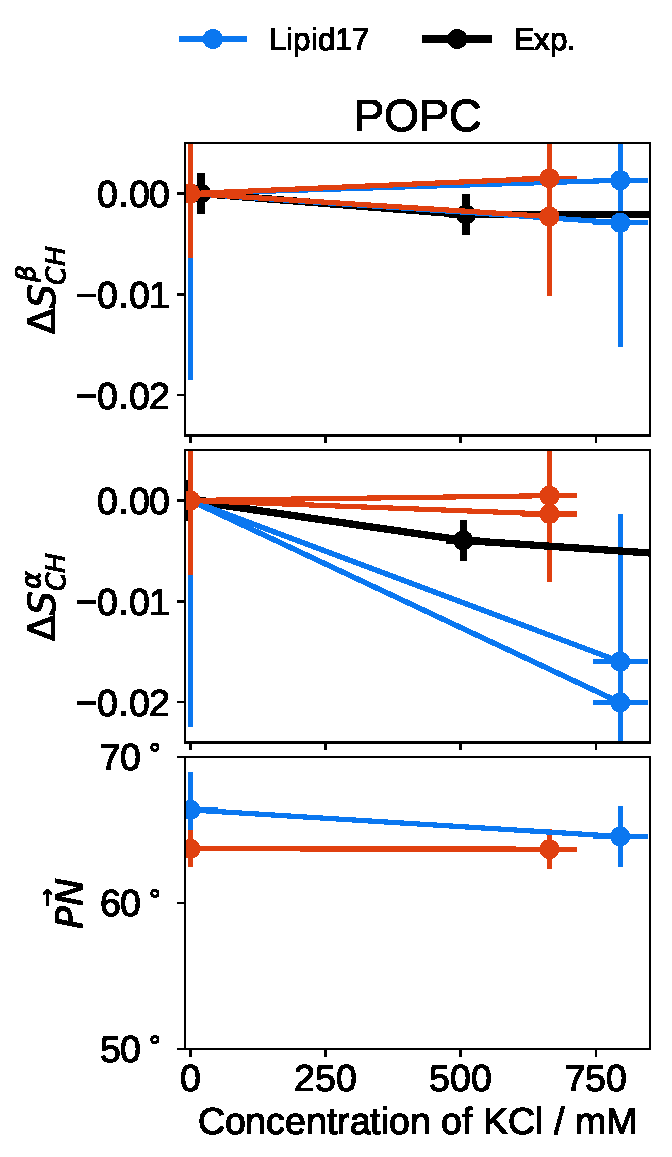
\includegraphics[height=\figheightsmall]{../img/ecc_pops/order_parameters_changes_ecc-lip_L14_A-B-PN-COO_POPC_kcl.pdf} 
  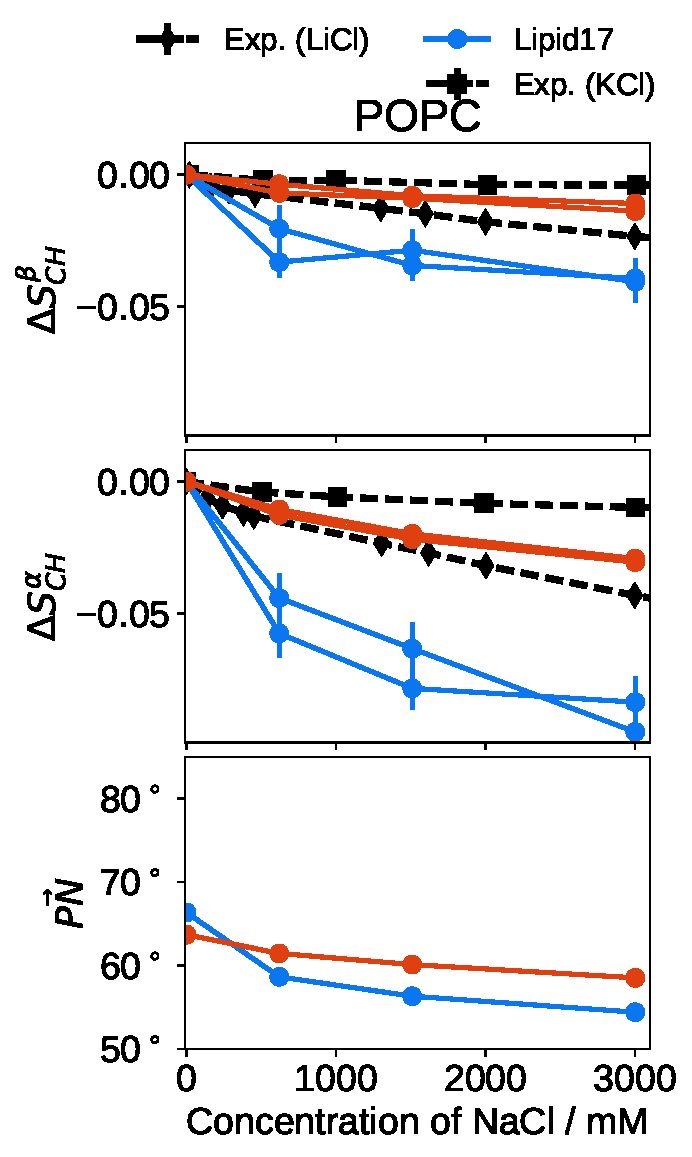
\includegraphics[height=\figheightsmall]{../img/ecc_pops/order_parameters_changes_ecc-lip_L14_A-B-PN-COO_POPC_nacl.pdf} 
  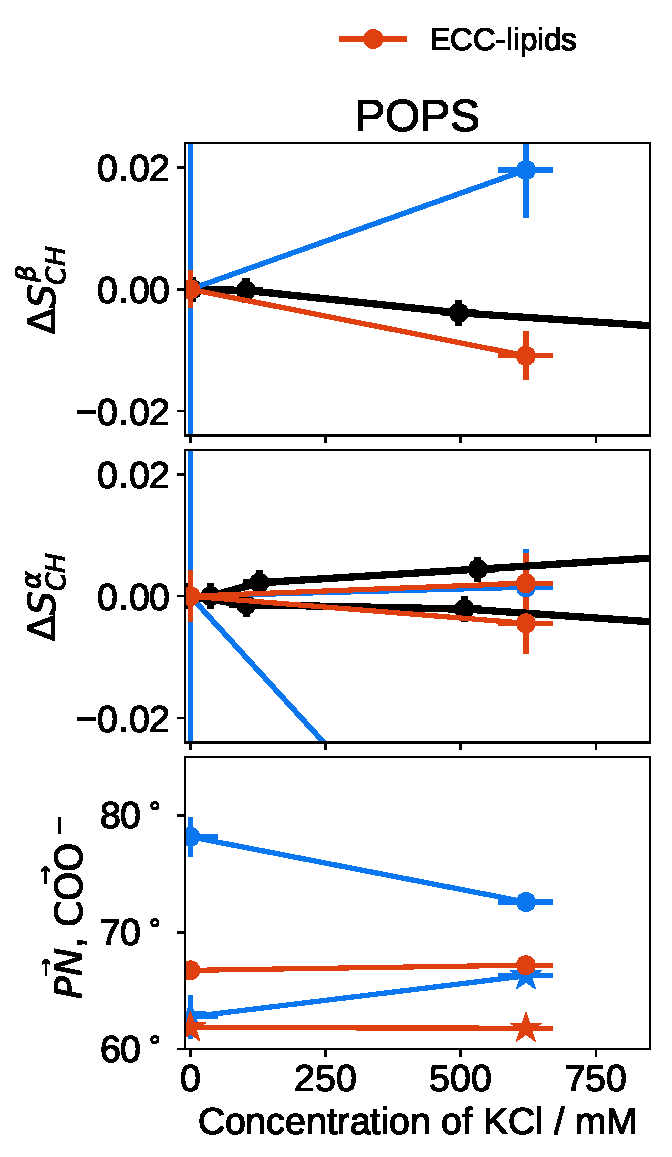
\includegraphics[height=\figheightsmall]{../img/ecc_pops/order_parameters_changes_ecc-lip_L14_A-B-PN-COO_POPS_kcl.pdf} 
  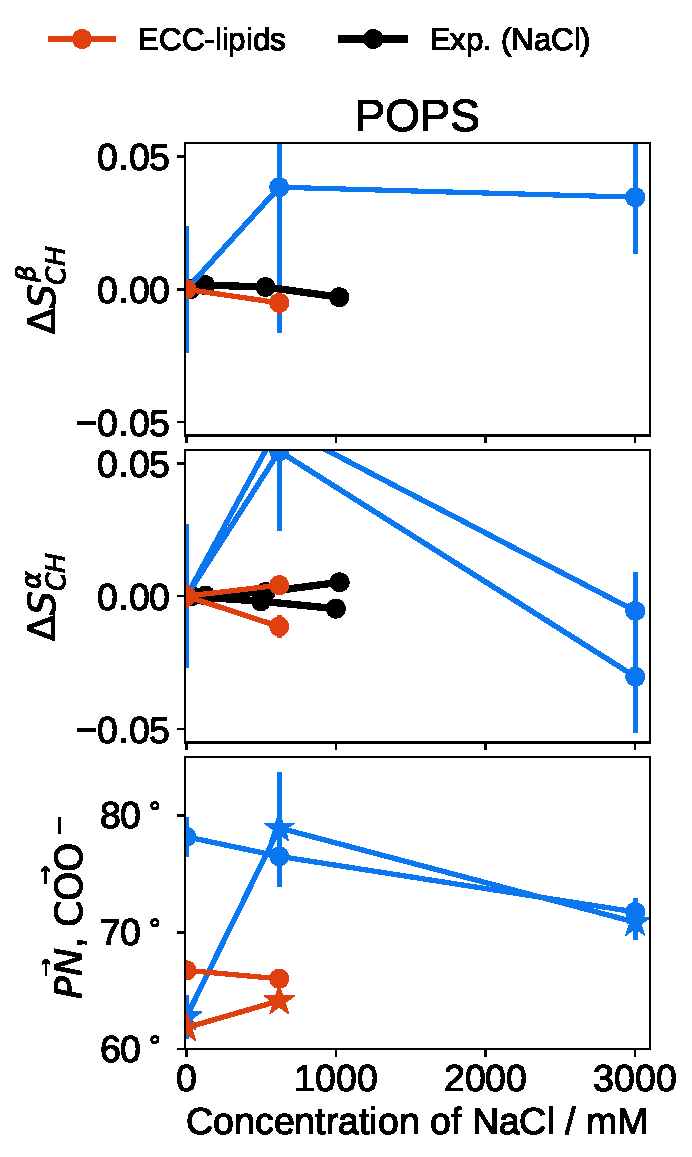
\includegraphics[height=\figheightsmall]{../img/ecc_pops/order_parameters_changes_ecc-lip_L14_A-B-PN-COO_POPS_nacl.pdf} 
  \caption{\label{fig:delta_ordPar_monoval_PCPS}
    Changes of the head group order parameters, and the angles of P--N and \ce{C_\beta-C_\gamma} (stars) vectors 
    with respect to the membrane normal of POPC (left) and POPS (right) in a POPC:POPS (5:1) bilayer 
    as a function of \ce{KCl} and \ce{NaCl} concentration from ECC-lipids and Lipid17/Dang simulations 
    compared with experimental values from Ref. \citenum{roux90} (signs from Ref. \citenum{ferreira16}) at 298 K.
    The y-axis for the $\alpha$-carbon results of POPS (middle right) is transferred
    with the same value for both order parameters such that the lower order
    parameter value from pure POPS is at zero to correctly illustrate the significant forking.
    Because experimental data with \ce{NaCl} is not available for POPC, the data for KCl and \ce{LiCl} (dashed line, left)
    are shown as lower and upper bounds, respectively, for the response to \ce{NaCl}.
    Error bars are not visible for ECC-lipids simulations because they are smaller than the point size.
  }
\todo{J: Will improve this figure with panels A, B, C and D 
and put POPC together, POPS together 
and remove the duplicate y-axis titles 
and make a common legend distinguishing different experiments better. }
\todo{The scale in left and right columns (response to KCl and NaCl) should be the same (not necessarily the same scale for POPC and POPS though).}
\end{figure} 


In experiments, the addition of K$^+$ ions led to a very modest decrease of POPC headgroup order parameters in POPC:POPS (5:1) mixture,
while the decrease was more pronounced with Li$^+$ ions and was strongest with divalent Mg$^{2+}$ and Ca$^{2+}$ ions~\cite{roux90},
suggesting that the binding affinity increases in order K$^{+}$ $<$ Li$^{+}$  $<$ Mg$^{2+}$  $<$ Ca$^{2+}$.
The small changes of POPC headgroup order parameters with increasing amount of KCl are close to experiments
%and the change in P--N vector is negligible
in both force fields (Fig.~\ref{fig:delta_ordPar_monoval_PCPS}).
The slightly overestimated change of the $\alpha$-carbon
order parameter in the Lipid17/Dang simulations may be due to the
deeper penetration of \ce{K+} into the bilayer (Fig.~\ref{fig:delta_ordPar_NaCl_PC-PS_mix_PC}).
Experimental data with the additional amount of \ce{Na+} in POPC:POPS (5:1) mixture is not available,
%we compared the simulation results to the experimental data with the additional amounts of
but \ce{Li+} and \ce{K+} results give the lower and the upper bounds, respectively, to the sodium binding
affinity (Fig.~\ref{fig:delta_ordPar_monoval_PCPS}). In ECC-lipids simulations,
the response of POPC headgroup order parameters to the additional sodium is close to the
experimental results for lithium, while in Lipid17/Dang simulations the response is larger.
% The following conclusion is already in the previous sentence, so I commented it out
Overall, the results suggest that the \ce{Na+} binding affinity is
% (Fig. \ref{fig:POPS-counterions-dens})
%and the tilting of P--N vector more perpendicular to the membrane surface (Fig. \ref{fig:delta_ordPar_NaCl_PCPS})
clearly overestimated in Lipid17/Dang simulations and slightly overestimated in ECC-lipids simulations,
while the binding affinity of potassium is better described by both force fields.
%First, we monitor the response of POPC headgroup order parameters to the increasing amount of POPS (Fig.~\ref{fig:delta_ordPar_NaCl_PC-PS_mix_PC}).
This conclusion is also supported by the POPC headgroup responses to the
increasing amount of POPS in different simulations (Fig~\ref{fig:delta_ordPar_NaCl_PC-PS_mix_PC}).
In experiments,
the head group order parameters of PC lipids increase upon addition of
% with the increasing amount of
negatively charged PS lipids, as predicted by the electrometer concept~\cite{seelig87,scherer87}.
%, because the headgroup P--N dipole
%tilts more parallel to the membrane interface \cite{seelig87,scherer87}.
This is the case also in simulations with the exception of
Lipid17/Dang with \ce{Na+} counterions, where the
%but not with \ce{Na+} counterions,
%However, in simulations with
stronger counterion binding affinity
%, the charge of bound
%counterions
cancels the influence of negatively charged lipids and the increase in PC headgroup
order parameters is not observed.% \cite{NMRlipidsIV}.

%Lipid17/Dang ion simulations 
%while in simulations with \ce{K+} counterions and in

%The trend is observed with both force fields in simulations
%the counterion binding affinity is weaker and the
%order parameters increase as in experiments (Fig~\ref{fig:delta_ordPar_NaCl_PC-PS_mix_PC}).  
%In contrast, the order parameters are unchanged or decrease 
%and the P--N vector tilts more perpendicular to the membrane interface.
%in 
%The result can be explained by the higher binding affinity of sodium in the
%Lipid17/Dang ion simulations (Fig~\ref{fig:delta_ordPar_NaCl_PC-PS_mix_PC}), which
%compensates the negative charge of PS lipids at the interface.
%This is corrected in ECC-lipids, 
%which only slightly underestimate the slopes of the order parameters 
%when \ce{Na+} counterions are used (Fig.~\ref{fig:delta_ordPar_NaCl_PC-PS_mix_PC}). 
%According to the electrometer concept, the decrease of PC head group order parameters
%correlates with the amount of bound cations to lipid bilayer \cite{akutsu81,altenbach84,seelig87,roux90,catte16,NMRlipidsIV}.
%Second, we monitor the response of PC headgroup order parameters to the additional
%amount of \ce{NaCl} and \ce{KCl} in POPC:POPS (5:1) mixtures.





%\subsection{Molecular interaction and binding affinities of K$^+$ and Na$^+$ cations to mixed POPC:POPS (5:1) membrane} 
%\label{sec:K_Na_added} 
\begin{figure*}[!tbp] 
  \centering 
  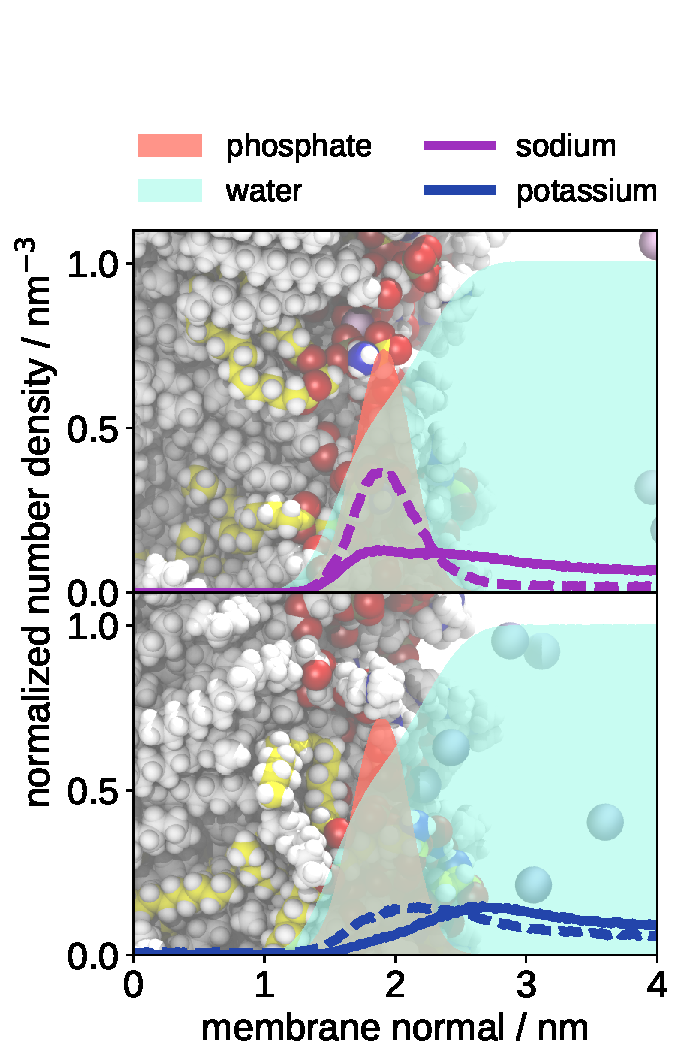
\includegraphics[height=\figheightsmall]{../img/ecc_pops/density_profiles_na-k-counterions_wat_phos_compar_5PC-1PS_ecclipids-lipid17.pdf}
  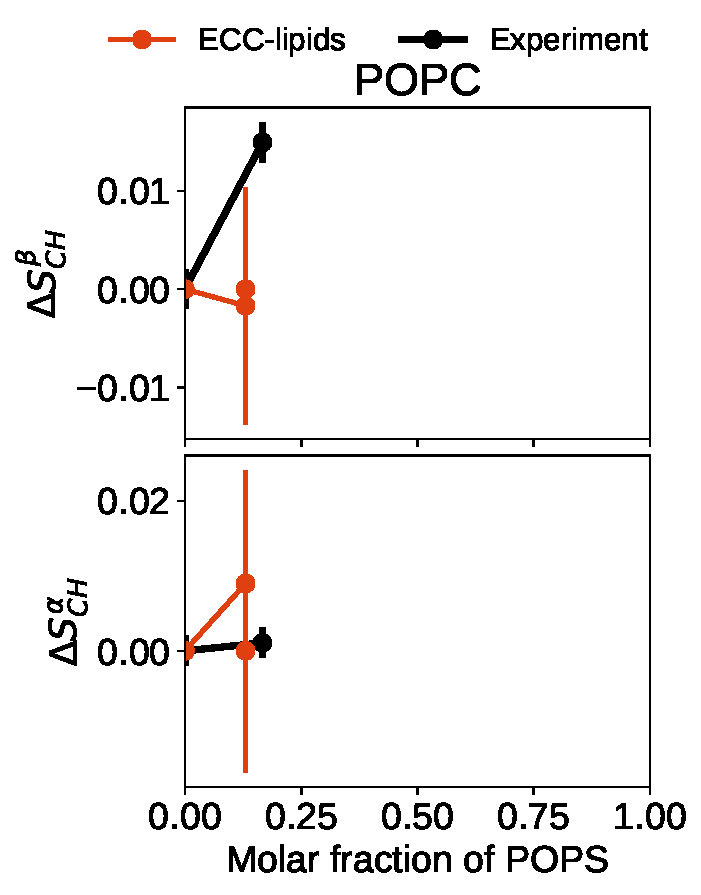
\includegraphics[height=\figheightsmall]{../Fig/order_parameters_changes_A-B_PC-PS_mix_POPC_nacl.pdf} 
  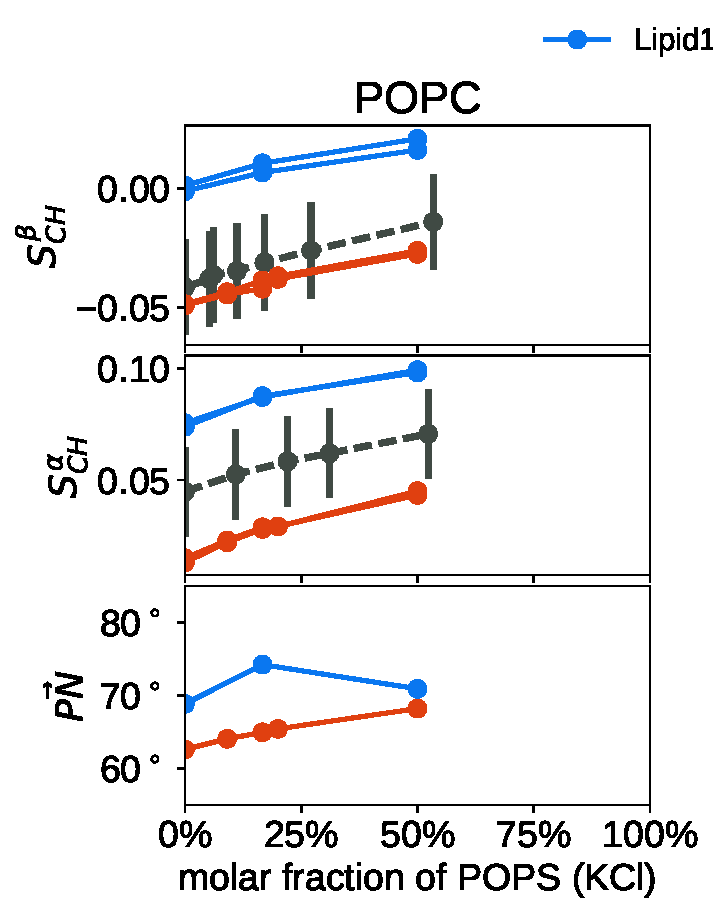
\includegraphics[height=\figheightsmall]{../Fig/order_parameters_changes_A-B_PC-PS_mix_POPC_kcl.pdf} 
  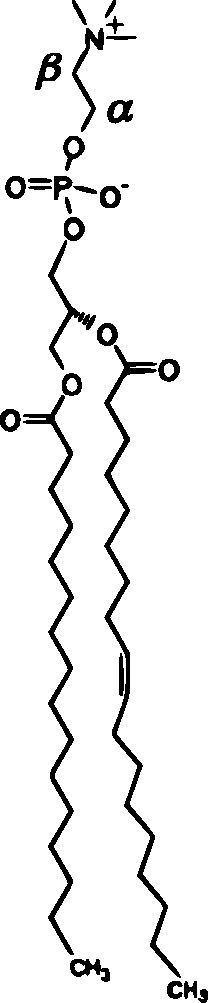
\includegraphics[height=\figheightsmall]{../img/POPCstructure.pdf} 
  \caption{\label{fig:delta_ordPar_NaCl_PC-PS_mix_PC} 
    \textbf{Left:} Number density profiles of \ce{K^{+}} and \ce{Na^{+}} counterions along the membrane normal axis
    in ECC-lipids (solid lines) and Lipid17/Dang (dashed lines) simulations of POPC:POPS (5:1) bilayers.  
    The density profiles of phosphate groups and water are divided by 4 and 100, respectively.  
    \textbf{Middle:} The POPC head group order parameters and the P--N vector angle
    with respect to the membrane normal as a function of POPS content in a bilayer
    from ECC-lipids and Lipid17/Dang simulations with \ce{Na^+} (left) and \ce{K^+} (right) counterions.
    Experimental order parameter values are from Ref. \citenum{scherer87}
    and the signs from Ref. \citenum{ferreira16} 
    (only \ce{Na^+} counterions, but shown also in the right plots for \ce{K+}).
    Error bars are not visible for most of the simulation points because they are smaller than the point size.
    \textbf{Right:} Chemical structure and labelling of carbon segments of POPC. 
  }
\todo{J: Will manually improve this figure with panels A, B, C and D 
and will erase the duplicate y-axis description 
and will add ticks to the right side of the plotting area. }
\todo{The scales should be the same in the left and right panel.}
\end{figure*} 


 
 


The behaviour of POPS headgroup can be further characterized by monitoring its order parameters in different
lipid mixtures and ionic conditions~\cite{NMRlipidsIV,roux90}.
Upon increasing the POPC content or monovalent ion concetration in experiments, 
the headgroup order parameters of POPS are almost unchanged
(\ref{fig:delta_ordPar_NaCl_PC-PS_mix_PS} and Figs.~\ref{fig:delta_ordPar_monoval_PCPS}).
%while calcium leads to relatively large changes with low concentrations followed by a rapid saturation below 100mM (Fig. \ref{fig:delta_ordPar_CaCl_PCPS}) \cite{scherer87,roux90}.
%The interaction with \ce{K^+}, which binds very weakly to both neutral and negatively charged membranes, 
%renders a qualitatively different response of the order parameter $S^\beta$ in POPS 
%in the mixed negatively charged bilayers compared to the neutral bilayers. 
%While the order parameter $S^\beta$ increases for both \ce{Na^+} and \ce{Ca^{2+}},
%it decreases in the presence of \ce{K^+}
%(\ce{KCl}:  Fig.~\ref{fig:delta_ordPar_KCl_PCPS}, 
% \ce{NaCl}: Fig.~\ref{fig:delta_ordPar_NaCl_PCPS}, and
%\ce{CaCl2}: Fig.~\ref{fig:delta_ordPar_CaCl_PCPS}). 
In Lipid17/Dang simulations, the changes of POPS headgroup order parameters with increasing amount of
both POPC or monovalent salts (\ce{KCl} and \ce{NaCl}) are overestimated (\ref{fig:delta_ordPar_NaCl_PC-PS_mix_PS} and Figs.~\ref{fig:delta_ordPar_monoval_PCPS}).
%These structural changes can relate to variations in the interactions between PC and PS head groups 
%and also to the changing amount of counterions and PS in the composition. 
%Also, the PS headgroup order parameters from simulations with Lipid17/Dang model
%are too sensitive to an additional amount of
%(Fig.~\ref{fig:delta_ordPar_monoval_PCPS}).
Similar results %The overestimation of the order parameter changes upon increasing amount of POPC in a bilayer 
also for other force fields are reported elsewhere~\cite{NMRlipidsIV}.
In ECC-lipids simulations, the response of POPS headgroup order parameters to both POPC and monovalent salt concentration (\ce{KCl} and \ce{NaCl})
are more modest and closer to experiments (\ref{fig:delta_ordPar_NaCl_PC-PS_mix_PS} and Figs.~\ref{fig:delta_ordPar_monoval_PCPS}).
The changes in order parameters can be related to the orientations of the P--N and C$_{\beta}$--C$_{\gamma}$
vectors in POPC and POPS, which change much less and more systematically in ECC-lipids
than in Lipid17/Dang simulations (\ref{fig:delta_ordPar_NaCl_PC-PS_mix_PS} and Figs.~\ref{fig:delta_ordPar_monoval_PCPS}). 

% where the changes in the PS headgroup orientation are more modest (Fig.~\ref{fig:delta_ordPar_NaCl_PC-PS_mix_PC}).
%In particular, 
%the dependence of the PS headgroup order parameters from ECC-lipids simulations
%to increasing amount of POPC, \ce{KCl} or \ce{NaCl}
%is weaker and closer to experiments 
%(Fig.~\ref{fig:delta_ordPar_monoval_PCPS}).
%In contrast, ECC-lipids with ECC-ions capture the different response 
%of the order parameters $S^{\beta}$, $S^{\alpha _1}$ and $S^{\alpha _2}$ in POPS 
%to various concentrations of \ce{NaCl} and \ce{KCl} in a good agreement with the experiments
%(\ce{KCl}:  Fig.~\ref{fig:delta_ordPar_KCl_PCPS}, 
% \ce{NaCl}: Fig.~\ref{fig:delta_ordPar_NaCl_PCPS}). 
%Such a dramatic improvement in the structural parameters 
%demonstrates that including electronic polarization in phospholipids is crucial 
%even for interactions with soft cations like \ce{K^+}. 

% This§: 
% adsorption and affinities of Na and K to PC:PS memb
% from densities and rel.surf.excess
% 
%in  Fig.~\ref{fig:POPS-counterions-dens} (only counterions)
%and Fig.~\ref{fig:nacl-dens_PCPS}        (additional salt concentrations), 
%
We estimate the influence of negatively charged POPS on the counterion binding affinity
% can be estimated 
%by calculating the amounts of phospholipids per bound \ce{Ca^{2+}} cation, $\xi _{Ca^{2+}}$,
by comparing the relative surface excesses with respect to water, $\Gamma ^{w} _{\rm ion}$,
between POPC:POPS (5:1) mixture and pure POPC in ECC-lipids simulations with the most realistic
cation binding affinities~\cite{melcr18}.
%Threshold for counting bound \ce{Ca^{2+}} cations to a membrane
%was set to $0.3\,\mathrm{nm}$ from oxygen atoms in lipids as in Ref.~\citenum{melcr18}.  
%Such a quantity compares the adsorption of ions to the adsorption of water molecules at an interface 
%without the necessity of defining a Gibbs dividing surface. \citep{melcr18, chattorajBOOK}
The value of $\Gamma ^{w} _{\rm Na}=-0.11 \pm 0.01 \mathrm{nm}^{-2}$ for 1~M sodium in pure ECC-POPC
simulation was reported in the previous work \cite{melcr18}.
The presence of $\sim$17\% POPS in a POPC bilayer increases the
%relative surface excess of sodium with respect to water from negative
value to $\Gamma ^{w} _{\rm Na}=0.092 \pm 0.005 \mathrm{nm}^{-2}$ 
for 0.621 M sodium, while value for potassium remains negative,
$\Gamma ^{w} _{\rm K}=-0.123 \pm 0.005 \mathrm{nm}^{-2}$ in POPC:POPS (5:1) mixture (Fig.~\ref{fig:nacl-dens_PCPS}).
As discussed above, the sodium binding to POPC:POPS (5:1) mixture may be slightly overestimated also in
ECC-lipids simulations. The response of headgroup order parameters to the addition of NaCl are
slightly overestimated also in ECC-POPC simulations (Fig 3 in Ref. \citenum{melcr18}),
suggesting that similar small overestimation of sodium binding may also occur to a pure POPC bilayer.
Therefore, the overestimation may arise from the sodium interactions with PC headgroup and
increase in binding affinity due to PS lipids would not be affected.
%Interestingly enough, \ce{K^+} maintains negative values of $\Gamma^{w}_{K}$ even for the negatively charged PC:PS~(5:1) bilayer.
%This is also evident from the density plots in  Fig.~\ref{fig:nacl-dens_PCPS}
%showing that the density profile of \ce{K^+} along the membrane normal 
%decays clearly faster towards the membrane centre compared to the density of water. 
%In contrast, the density profile of \ce{Na^+} has a shoulder 
%at the region of the phosphate groups,
%which demonstrates that sodium cations adsorb weakly to the membrane interface compared to the aquaeous solution
%by yielding a small positive value of $\Gamma^{w}_{Na}$.



\subsection{Molecular interaction and binding affinity of \ce{Ca^{2+}} cations to mixed POPC:POPS (5:1) membrane} 
\label{section:lip-ion_ca}

%The headgroup order parameters of PC lipids decrease more upon addition of \ce{CaCl2}
%in POPC:POPS (5:1) mixtures than in pure PC bilayers due to the higher calcium binding
%affinity to the negatively charged lipid bilayers \cite{akutsu81,altenbach84,roux90,NMRlipidsIV}.
Our recent work demonstrates that the POPC headgroup order parameters measured
from POPC:POPS (5:1) mixture as a function of CaCl$_2$ concentration 
can be used to evaluate the calcium binding affinity to lipid bilayers containing PS lipids \cite{roux90, NMRlipidsIV}.
The decrease of the PC headgroup order parameters in this mixture upon addition of \ce{CaCl2} 
were overestimated by the Lipid17/Dang simulations (also shown in Fig.~\ref{fig:delta_ordPar_CaCl_PCPS})
and all other tested force fields except CHARMM36 with the recently introduced NBfix for calcium \cite{kim16},
which underestimated the headgroup order parameter response.
In ECC-lipids simulations, the headgroup responses are in better agreement with experiments (Fig.~\ref{fig:delta_ordPar_CaCl_PCPS}),
indicating that the lower binding affinity than in Lipid17/Dang simulations is more realistic (Fig.~\ref{fig:cacl-dens_PCPS}).
%However, the steep decrease of the order parameters at low calcium concentrations,
%observed especially in negatively charged bilayers \cite{borle85,macdonald87,roux90},
%may not be fully captured by the ECC-lipids simulations.
Therefore, we use ECC-lipids simulations to estimate the influence of negative charged POPS on
calcium binding affinity to lipid bilayers.
%containing PS lipids is illustrated in
%ECC-lipids simulations by the increasing
The relative surface excess of calcium with respect to water 
%  previously we used 350mM conc, but I think it is better to compare to a higher concentration to support the whole argument bullet-proof
%  $\Gamma^{w}_{Ca} = 0.06\mathrm{nm^{-2}}$ ($\sim ?.?$ phospholipids per bound \ce{Ca^{2+}}) for pure POPC bilayer with 346~mM CaCl$_2$ \cite{melcr18, ECC-POPC_nacl_cacl2_files} 
$\Gamma^{w}_{Ca} = 0.09\mathrm{nm^{-2}}$ ($\sim 5.4$ phospholipids per bound \ce{Ca^{2+}}) for pure POPC bilayer with 467~mM CaCl$_2$ \cite{ECC-POPC_nacl_cacl2_files}
is increased to
$\Gamma^{w}_{Ca} = 0.24\mathrm{nm^{-2}}$ ($\sim 4.8$ phospholipids per bound \ce{Ca^{2+}}) for the POPC:POPS (5:1) bilayer with 409 mM CaCl$_2$.
Besides lower binding affinity, ECC-lipids simulations yield smaller error bars for order parameters and shorter residence times (Fig.~\ref{fig:hist_residence_times}) 
than those typically observed in simulations with other force fields \cite{javanainen17,melcr18,NMRlipidsIV},
suggesting that the ECC accelerates the equlibration of ions at lipid bilayer interface.
Therefore, our 1 $\mu$s simulations seem to be sufficiently long for the ECC-lipids simulations, because
90\% of the calcium residence times are shorter than $60\,\mathrm{ns}$ for pure POPC bilayer
and shorter than $200\,\mathrm{ns}$ for POPC:POPS (5:1) mixture, while the
longest observed residence times are $141\,\mathrm{ns}$ and $485\,\mathrm{ns}$, respectively (Fig.~\ref{fig:hist_residence_times}).
Interestingly, the calcium residence times are 3-4 times longer in POPC:POPS (5:1) mixture than in pure POPC.


\begin{figure}[tbp!] 
  \centering 
  \begin{tabular}{ c }
  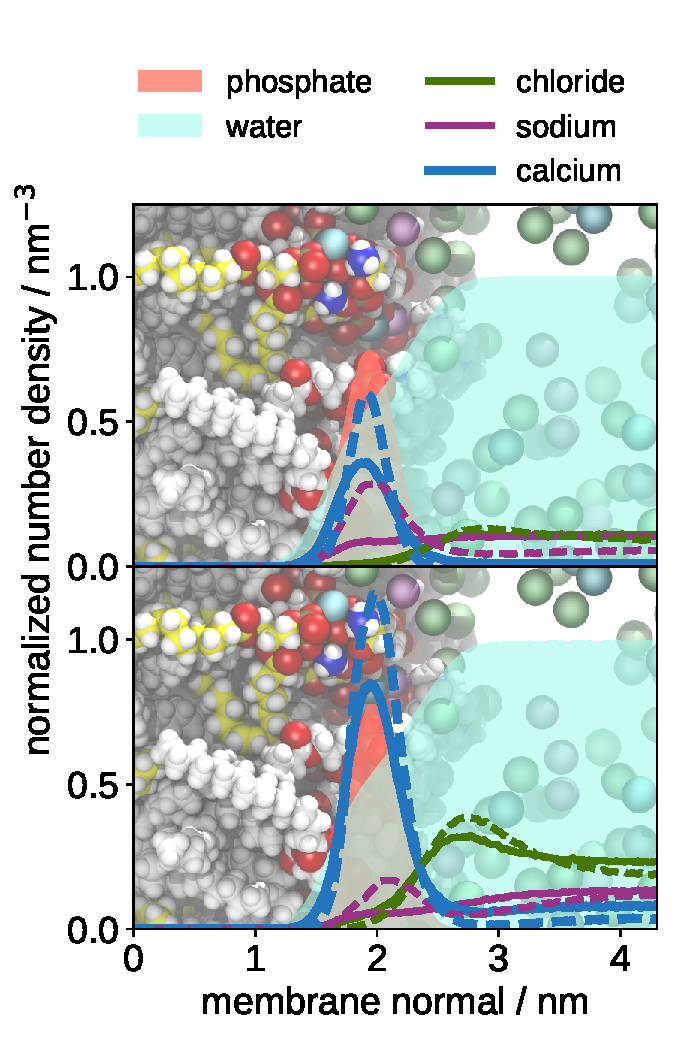
\includegraphics[height=1.5\figheightsmall]{../img/ecc_pops/density_profiles_ca_na_k_cl_wat_phos_ecclipids_lipid17_compar_80and200mMCaCl2.pdf}
  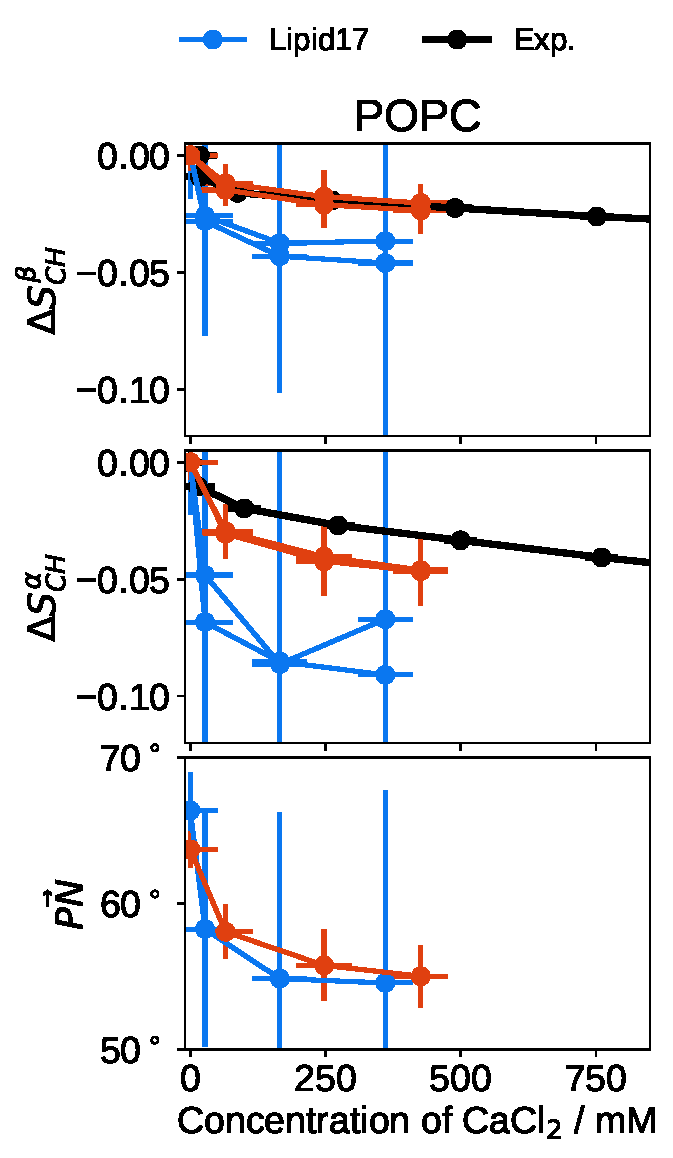
\includegraphics[height=1.5\figheightsmall]{../img/ecc_pops/order_parameters_changes_ecc-lip_L14_A-B-PN-COO_POPC_cacl.pdf} 
  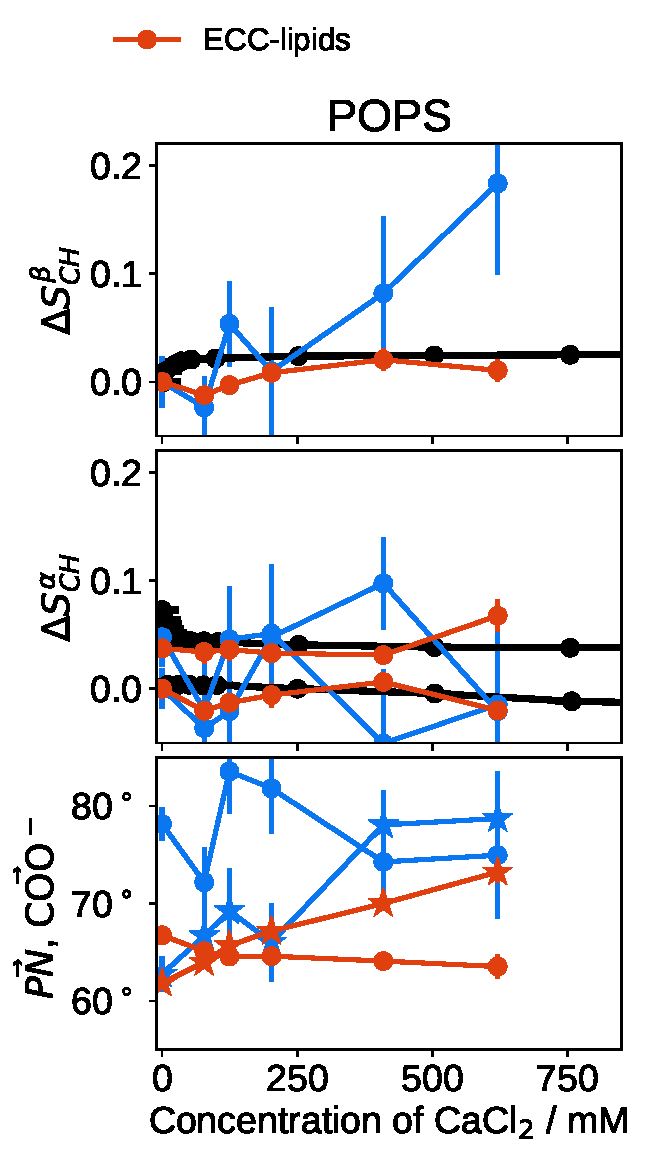
\includegraphics[height=1.5\figheightsmall]{../img/ecc_pops/order_parameters_changes_ecc-lip_L14_A-B-PN-COO_POPS_cacl.pdf} 
  \end{tabular}
%  \begin{tabular}{ c }
%  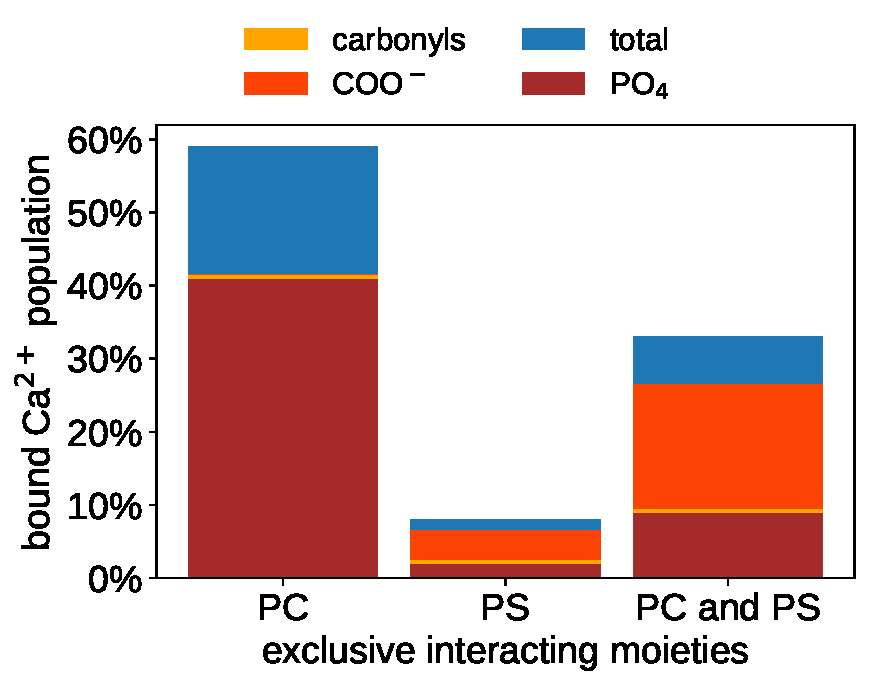
\includegraphics[width=3cm]{../img/bound_ca_populations.pdf} \\
%  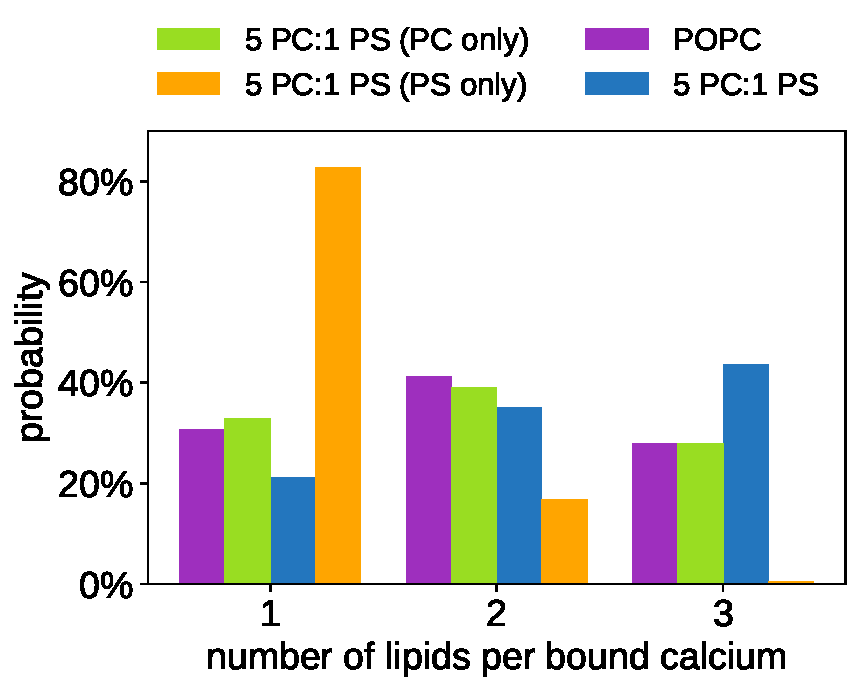
\includegraphics[width=3cm]{../img/stoichiometry_CaCl2_comparison_Ecc-lipids_PC-vs-PCPS.pdf} 
%  \end{tabular}
  \caption{\label{fig:cacl-dens_PCPS} 
    \textbf{Left panel:}
    Number density profiles of \ce{Ca^{2+}} and \ce{Cl^-} ions and \ce{Na^{+}} counterions 
    along the normal of the membrane starting at the centre
    for the negatively charged membrane with the composition 5\,PC:1\,PS
    at 80~mM (top) and 200~mM (bottom) added buffer concentrations of \ce{CaCl2} from simulations with ECC-lipids (solid) and Lipid17 (dashed). 
    In order to visualize the density profiles with a comparable scale 
    the density profile of~\ce{Ca^{2+}} ions are divided by 2, and 
    the density profiles of phosphate groups and water are divided by 4 and 100, respectively.  
  }
  \caption{\label{fig:delta_ordPar_CaCl_PCPS} 
    \textbf{Middle panels:}
    Changes of the head group order parameters, and the angles of P--N (circles) and C$_\beta$--C$_\gamma$ (stars) vectors 
    with respect to the membrane normal of POPC (left) and POPS (right) in a POPC:POPS (5:1) bilayer 
    as a function of \ce{CaCl$_2$} concentration from ECC-lipids and Lipid17/Dang simulations 
    compared with experimental values from Ref. \citenum{roux90} (signs from Refs. \citenum{ferreira16} and \citenum{NMRlipidsIV}) at 298 K.
    The y-axis for the $\alpha$-carbon results of POPS (middle right) is transferred
    with the same value for both order parameters such that the lower order
    parameter value from pure POPS is at zero to correctly illustrate the significant forking.
    Error bars are not visible for ECC-lipids simulations because they are smaller than the point size.
  }
%  \caption{ \label{fig:cacl_complexes} 
%    \textbf{Right top:} Percentages of the bound Ca$^{2+}$ 
%    in exclusive contact with the given oxygen moiety
%    when bound to PC only, PS only or simultaneously to both
%    calculated from ECC-lipids simulation of POPC:POPS (5:1) bilayer with 409 mM CaCl$_2$. 
%%	The areas represent populations of bound \ce{Ca^{2+}} 
%%	only to the given moieties exclusively (shades of orange and red)
%%	or their combinations (CHANGE:blue)
%%	separately for PC, PS, or PC and PS simultaneously. 
%%	The areas sum up to total populations at the respective lipids. %
%	In the case of simultaneous binding to both PC and PS%,
%	the percentages refer to the moieties in PS.
%	% i.e., PC can interact with any considered moiety.
%        For numerical values, see table~\ref{tab:binding}.
%    \textbf{Right bottom:} Relative probabilities of \ce{Ca^{2+}} ions to coordinate with a certain number of lipids
%    in pure POPC bilayer with 350 mM CaCl$_2$ and in POPC:POPS (5:1) mixture with 400 mM CaCl$_2$.  
%    Analysis was done for both systems by considering all lipids (blue and violet) and
%    for POPC:POPS (5:1) mixture also by considering POPC and POPS lipids separately (green and orange). 
%    %All lipids were taken into account with the exception of the complexes in light green and orange, 
%    %for which we counted only contacts with POPC resp POPS from the mixed 5\,PC:1\,PS negatively charged bilayer. 
%    %The calculated probabilities of the calcium-lipid complexes also reflect only POPC (light green) resp POPS (orange). 
%    % Probabilities were taken from simulations with comparable bulk concentrations of calcium around 250~mM. 
%    Clusters of four or more lipids were not observed in either membrane.
%    The threshold for counting coordinated lipids in a complex with \ce{Ca^{2+}} was set to $0.3\,\mathrm{nm}$, 
%    as the distance between the cation and the oxygen atoms of the lipids. 
%    Previously published simulation data \cite{melcr18} for pure POPC bilayers were taken directly from \cite{ECC-POPC_nacl_cacl2_files}. 
%  }
  \todo{J: Will adjust the Fig into a nice panel and change the captions accordingly. } \\
\end{figure}

% SAMULI: I separated the figure below, because it was too small to be read when combined with others.
% It might be too much to all of these into the same.

\begin{figure}[tbp!] 
  \centering 
  \begin{tabular}{ c }
  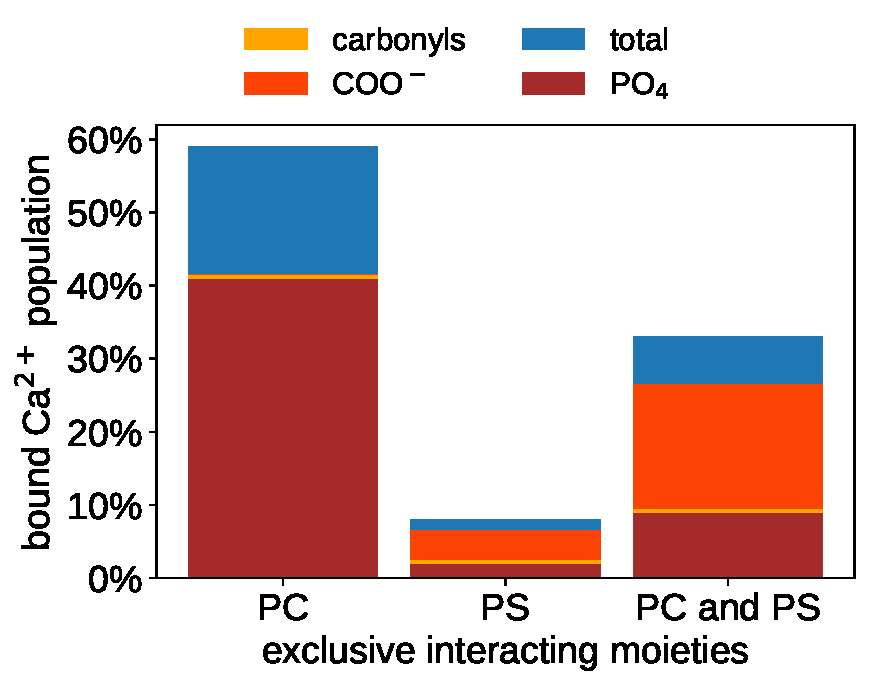
\includegraphics[width=8cm]{../img/bound_ca_populations.pdf} \\
  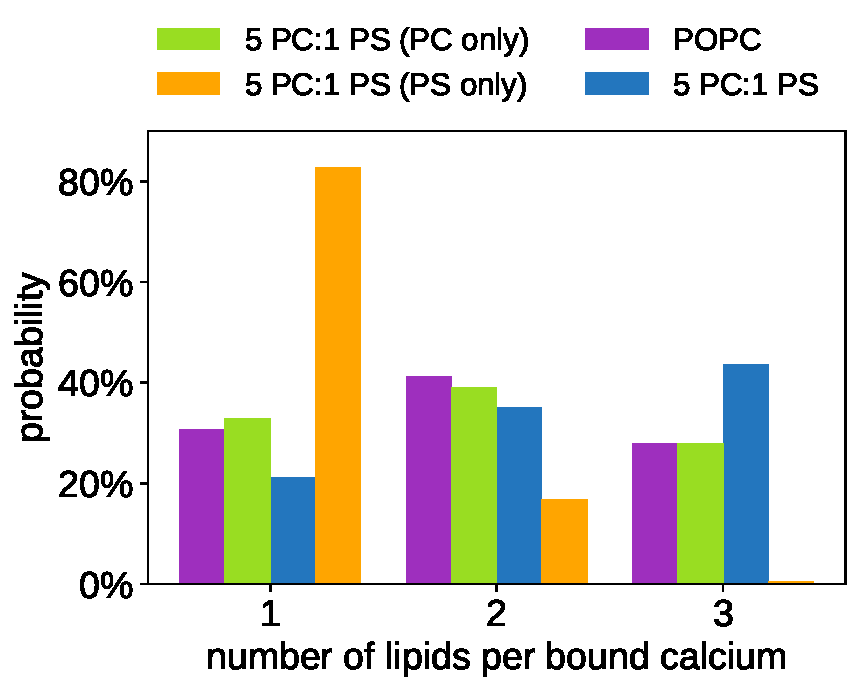
\includegraphics[width=8cm]{../img/stoichiometry_CaCl2_comparison_Ecc-lipids_PC-vs-PCPS.pdf} 
  \end{tabular}
  \caption{ \label{fig:cacl_complexes} 
    \textbf{Top:} Percentages of the bound Ca$^{2+}$ 
    in exclusive contact with the given oxygen moiety
    when bound to PC only, PS only or simultaneously to both
    calculated from ECC-lipids simulation of POPC:POPS (5:1) bilayer with 409 mM CaCl$_2$. 
%	The areas represent populations of bound \ce{Ca^{2+}} 
%	only to the given moieties exclusively (shades of orange and red)
%	or their combinations (CHANGE:blue)
%	separately for PC, PS, or PC and PS simultaneously. 
%	The areas sum up to total populations at the respective lipids. 
	In the case of simultaneous binding to both PC and PS,
	the percentages refer to the moieties in PS.
	% i.e., PC can interact with any considered moiety.
        For numerical values, see table~\ref{tab:binding}.
    \textbf{Bottom:} Relative probabilities of \ce{Ca^{2+}} ions to coordinate with a certain number of lipids
    in pure POPC bilayer with 350 mM CaCl$_2$ and in POPC:POPS (5:1) mixture with 400 mM CaCl$_2$.  
    Analysis was done for both systems by considering all lipids (blue and violet) and
    for POPC:POPS (5:1) mixture also by considering POPC and POPS lipids separately (green and orange). 
    %All lipids were taken into account with the exception of the complexes in light green and orange, 
    %for which we counted only contacts with POPC resp POPS from the mixed 5\,PC:1\,PS negatively charged bilayer. 
    %The calculated probabilities of the calcium-lipid complexes also reflect only POPC (light green) resp POPS (orange). 
    % Probabilities were taken from simulations with comparable bulk concentrations of calcium around 250~mM. 
    Clusters of four or more lipids were not observed in either membrane.
    The threshold for counting coordinated lipids in a complex with \ce{Ca^{2+}} was set to $0.3\,\mathrm{nm}$, 
    as the distance between the cation and the oxygen atoms of the lipids. 
    Previously published simulation data \cite{melcr18} for pure POPC bilayers were taken directly from \cite{ECC-POPC_nacl_cacl2_files}. 
  }
  \todo{Bottom: The x-axis label should be changed to ''number of lipids directly bound to Ca$^{2+}$''.
    The current label has another meaning in the text now.}
  \todo{Bottom: The labels could be more clear. Maybe ''PC in POPC:POPS(5:1)'' ...}
\end{figure} 

Interactions between Ca$^{2+}$ ions and PS lipids can be further characterized by monitoring
the POPS headgroup order parameters from POPC:POPS (5:1) mixture with increasing  CaCl$_2$ concentration~\cite{roux90}.
In experiments, the headgroup order parameters of POPS exhibit a strong dependence
on low CaCl$_2$ concentrations with a rapid saturation below 100~mM  (Fig.~\ref{fig:delta_ordPar_CaCl_PCPS}) \cite{roux90}.
These changes are overestimated in simulations with Lipid17/Dang (Fig.~\ref{fig:delta_ordPar_CaCl_PCPS})
and other tested force fields in our recent work \cite{NMRlipidsIV}, 
including CHARMM36 with the NBfix correction for calcium
which underestimated the binding affinity.
In ECC-lipids simulations, the changes of the PS headgroup order parameters are not overestimated,
but the strong dependence on low concetrations of CaCl$_2$ is not fully reproduced (Fig.~\ref{fig:delta_ordPar_CaCl_PCPS}).
In addition to possibly suboptimal interactions between calcium ions and PS headgroup, the potential sources of this
discrepancy include the above observed sligth overestimation of \ce{Na^+} counterions and
imperfect structures of the lipid headgroup (Fig.~\ref{simVSexpNOions_POPS}).
The POPS headgroup order parameters are also related to the changes of average orientation of P--N and
C$_{\beta}$--C$_{\gamma}$ vectors in the PS headgroup, which are smaller and more systematic
in ECC-lipids than in Lipid7/Dang simulations (Fig.~\ref{fig:delta_ordPar_CaCl_PCPS}).
Upon addition of 620~mM CaCl$_2$ to POPC:POPS (5:1) mixture,
the average orientation of P--N vectors in both POPC and POPS headgroups tilts more perpendicular to the membrane surface
by 11$^\circ$ and  3$^\circ$, respectively, in ECC-lipids simulations (Fig.~\ref{fig:delta_ordPar_CaCl_PCPS}),
suggesting that the PS headgroup orientation is less sensitive to the bound calcium than PC.
On the other hand, the average orientation of the C$_{\beta}$--C$_{\gamma}$ vector in PS headgroup
tilts to the opposite direction by $11^\circ$ in the same system.
%In Lipid17/Dang simulations, the changes in both headroup orientations and order parameters
%are larger and less systematic for the PS headgroup, especially with lower concentrations (Fig.~\ref{fig:delta_ordPar_CaCl_PCPS}).

%SAMULI: We will not go to the spin relaxation time analysis in this work
%and average angles do not give information about dynamics
%
%It has been pointed out in previous experimental works
%that the conformational flexibility of PS head groups 
%is different from other lipids \cite{browning80}. 
%While the static shielding tensor of PS is not substantially different from PC or PE, 
%the $^{31}$P~$T_1$ relaxation times are significantly shorter for PS. 
%It is suggested that the PS head group is more rigid compared to the other phospholipids, 
%which is also corroborated by a larger chemical shielding anisotropy of PS \cite{browning80}. 


Recent analyzes of interaction sites between calcium and PS lipids combining
MD simulations with various experimental techniques have been 
controversial because the results strongly depend on force fields parameters \cite{melcrova16,valentine18,hallock18}.
Here, we analyze the calcium binding details from ECC-lipids simulation of POPC:POPS (5:1) mixture with 409 mM CaCl$_2$,
because it surpasses the quality of other force fields in direct comparison with experimental order parameter data.
In the ECC-lipid simulation, calcium ions binds approximately twice more likely 
to the carboxylate than to the phosphate moiety of POPS headgroup,
while binding to acyl chain carbonyls is almost negligible (Fig.~\ref{fig:cacl_complexes} and table~\ref{tab:binding}).
The result is consistent with CHARMM36 simulations without the NBfix correction \cite{hallock18},
but CHARMM36 simulations with the NBfix correction \cite{kim16} predict almost exclusive binding on carboxylate group \cite{valentine18}
and Berger simulations signifincant binding affinity also on acyl chain carbonyls \cite{melcrova16}.
On the other hand, calcium ions bind too strongly on bilayers simulated using CHARMM36 without the NBfix correction
or Berger models, and too weakly on CHARMM36 bilayers with the NBfix correction \cite{catte16,NMRlipidsIV}.
Furthermore, in CHARMM36 simulations without the NBfix,
calcium ions coordinate with even four distinct PS lipids \cite{hallock18}, while coordination with more than two PS lipids
was very rare in our ECC-lipids simulations (Fig.~\ref{fig:cacl_complexes}).
%Furthermore, the POPS:POPC:Ca$^{2+}$ (7:3:7) mixture with relatively high
%PS lipid fraction and calcium concentration was used in the previous work \cite{hallock18},
%which may lead to the complexation of \ce{Ca^{2+}} cations and PS lipids that is
%not observed with lower PS content used in ECC-lipids simulations in this work \cite{hauser77,kurland79,hauser85,feigenson86,mattai89,roux90,roux91}.
%While POPC interacts with the calcium cations almost entirely through its phosphate group 
%in both neutral \cite{melcr18} and negatively charged membranes, 
%the inteaction with POPS lipids happens more through the \ce{COO^-} group than through the \ce{PO4} group. 
%Interactions of \ce{Ca^{2+}} with carbonyl groups are also present for both POPC and POPS,
%however, they are always accompanied by interactions with phosphate groups. 

%Significant coordination of calcium with carbonyl groups of PS and PC lipids observed in previous
%simulations with the Berger force field \cite{melcrova16} %\cite{berger97,mukhopadhyay04}
%was not observed in ECC-lipids simulations in here nor in the previous work with pure POPC \cite{melcr18}.
%Overestimated coordination of cations with carbonyl groups is a potential source for
%the overestimated cation binding in Berger force field \cite{catte16,NMRlipidsIV}. 
%In CHARMM36 simulations with the NBfix, calcium mainly interacted with only
%carboxylate of PS lipids  \cite{valentine18}, which is a potential source for the
%underestimated calcium binding affinity to lipid bilayer with this force field \cite{NMRlipidsIV}. 

%on average 41\% of the total population of bound calcium cations is in contact with PS lipids
%with 8\% bound exclusively only to them even though the negatively charged membrane contains only 17\% of POPS (Fig.~\ref{fig:cacl_complexes}).
%%Therefore, calcium ions bind more likely to negatively charged PS lipids than neutral PC lipid in a mixed bilayer, as expected.
%	For comparison, in a pure POPC bilayer with 350 mM CaCl$_2$, 
%	67\% of bound \ce{Ca^{2+}} is exclusively in contact with \ce{PO_4} group. \cite{melcr18} 


%This can explain the diminished flexibility of the PS head group 
%from simultaneous binding of \ce{Ca^{2+}} to the \ce{COO^-} group in PS and a phosphate group in PC 
%as the most probable configuration (Fig.~\ref{fig:cacl_complexes}). 

%In contrast, the combination of NMR experiments 
%and MD simulations with the same model, CHARMM36, but without the correction for calcium binding
%also reveal long-lived interactions of \ce{Ca^{2+}} with \ce{PO4} groups. \cite{hallock18}
%Although the ratios of the life times of coordination follow the same trends as in our work,
%the lengths of simulation trajectories are insufficient 
%to yield converged results in this aspect (see SI and Refs.~\cite{catte16, melcr18, NMRlipidsIV}). 

\section{Conclusions} 
We have applied ECC to implicitly include electronic polarization to the Amber Lipid17 force field
parameters of negatively charged POPS lipid.
Because PS headgroup bears a unit negative charge, we apply the scaling factor of 0.75,
derived for monovalent ions~\cite{leontyev09}, to the partial charges
in the headgroup, glycerol backbone and carbonyl regions of POPS.
Following our previous work for zwitterionic POPC lipids, the 
Lennard-Jones $\sigma$ parameters of the same POPS segments were
scaled by a factor of 0.89 to optimize the hydration properties of the bilayer~\cite{melcr18}.
Similarly to other state of the art lipid models, the created ECC-POPS parameters give
lipid bilayer dimensions and acyl chain structures in agremeement with experiments,
but leaves room for improvement for the headgroup structure when validated against
NMR and scattering experiments~\cite{botan15,ollila16}.
Nevertheless, ECC-lipid parameters describe cation (Na$^+$ and Ca$^{2+}$) binding affinities
and their interactions with PS headgroups better than other available lipid force fields,
when validated using the headgroup order parameters and ``electrometer concept''~\cite{NMRlipidsIV}.
There is, however, room for improvement in capturing the sensitive headgroup responses to the
small concentrations of CaCl$_2$.

%Although the ECC-lipids model gives the most realistic picture of calcium binding to
%lipid bilayers containing PS lipids with respect to NMR order parameters, 


%The scaling factor for the charge
%We have developed a classical MD model of POPS, ECC-POPS, 
%which accurately describes features of both pure POPS membrane and its mixes with POPC. 
%This was achieved by applying ECC which accounts for electronic polarization. 
%Applying ECC to POPS lipids improves cation binding affinity to membranes
%mixed with POPC and also the response of PS headgroup to the bound cations.


In our ECC-lipids simulation, Ca$^{2+}$ ions bind twice more likely to carboxylate groups
of PS headgroups than to phosphate groups, while binding to carbonyls is almost negligible.
Binding of Ca$^{2+}$ ions to more than two POPS lipids simultaneously is very rare in ECC-lipids simulations.
Because ECC-lipids parameters give the best results in direct comparison with NMR order parameters, %used in this work is the direct connection between
we believe that our results help in resoving controversial interpretations of more indirect experiments
using different force fields~\cite{melcrova16,valentine18,hallock18}.
%measured and simulation data, which enables more unambiguous evaluation of the force field quality \cite{catte16,ollila16}
%than more indirect comparison in previous studies using 2D infrared spectroscopy \cite{valentine18}, NMR chemical shifts and
%rotational-echo double-resonance (REDOR) experiments \cite{hallock18} or fluorescent and vibrational sum frequency spectroscopy \cite{melcrova16}.
%Because the ECC-lipids model gives the best agreement with the experimental headgroup order parameters
%with various ion conctenrations among the available models, we believe that it also gives the currently best available
%interpretation of the experimental data. 
Furthermore, our results pave the way for more realistic MD simulations of anionic biological membranes,
and demonstrate the usefulness of ECC also for charged lipids.
\todo{Maybe Pavel could extend this by mentioning something that this is yet another case where ECC works and/or
  mentioning some concrete biological examples where anionic membrane/calcium interactions are important?}

%Therefore, further force field optimization is required for even more accurate MD simulations of cations
%in the vicinity of negatively charged lipid bilayers.



\listoftodos


% If you have acknowledgments, this puts in the proper section head. 
\begin{acknowledgement} 
% Put your acknowledgments here. 
P.J. acknowledges support from the Czech Science Foundation (grant no. 16-01074S)  
and from the Academy of Finland via the FiDiPro award. 
Computational resources were supplied by the Ministry of Education, Youth and Sports 
of the Czech Republic under the Projects CESNET (Project No. LM2015042) and CERIT-Scientific 
Cloud (Project No. LM2015085) provided within the program Projects of Large Research, 
Development and Innovations Infrastructures. 
O.H.S.O. acknowledges financial support from 
Integrated Structural Biology Research Infrastructure of 
Helsinki Institute of Life Science (Instruct-HiLIFE). 
\end{acknowledgement} 
 
\begin{suppinfo} 
 
%A listing of the contents of each file supplied as Supporting Information 
%should be included. For instructions on what should be included in the 
%Supporting Information as well as how to prepare this material for 
%publications, refer to the journal's Instructions for Authors. 
 
%The following files are available free of charge. 
%\begin{itemize} 
%  \item Filename: brief description 
%\end{itemize} 
 
\end{suppinfo} 
 
 
\bibliography{refs.bib} 
 
\end{document} 
 

